\documentclass[a4paper,11pt]{article}

\usepackage[portuguese]{babel}
\usepackage[utf8]{inputenc}
\usepackage{amsmath}
\usepackage{graphicx}
\usepackage{hyperref}
\usepackage{float}
\usepackage{subfig}
\usepackage{fixltx2e}
\usepackage[bottom]{footmisc}
\usepackage{listings}
\usepackage{xargs}                      % Use more than one optional parameter in a new commands
\usepackage[pdftex,dvipsnames]{xcolor}  % Coloured text etc.
\usepackage[colorinlistoftodos,prependcaption,textsize=tiny]{todonotes}
\newcommandx{\unsure}[2][1=]{\todo[linecolor=red,backgroundcolor=red!25,bordercolor=red,#1]{#2}}
\newcommandx{\change}[2][1=]{\todo[linecolor=blue,backgroundcolor=blue!25,bordercolor=blue,#1]{#2}}
\newcommandx{\info}[2][1=]{\todo[linecolor=OliveGreen,backgroundcolor=OliveGreen!25,bordercolor=OliveGreen,#1]{#2}}
\newcommandx{\improvement}[2][1=]{\todo[linecolor=Plum,backgroundcolor=Plum!25,bordercolor=Plum,#1]{#2}}
\newcommandx{\thiswillnotshow}[2][1=]{\todo[disable,#1]{#2}}
\usepackage[font=footnotesize]{caption}
\usepackage[hypcap]{caption}
\usepackage[top=2.5cm, bottom=2.5cm, left=2.5cm, right=2.5cm]{geometry}
\usepackage{enumerate}
%\usepackage[siunitx,american]{circuitikz}

\setcounter{tocdepth}{2}

\numberwithin{equation}{section}
\addto\captionsportuguese{\renewcommand{\contentsname}{Índice}}

\linespread{1.3}
\usepackage{indentfirst}

\begin{document}
\begin{titlepage}
\begin{center}

\hfill \break
\hfill \break


\includegraphics[width=0.3\textwidth]{img/logo}~\\[1cm] 

\textsc{\LARGE Instituto Superior Técnico}\\[0.25cm]
\textsc{\Large Mestrado Integrado em Engenharia Electrotécnica e de Computadores}\\[1.8cm]
\textsc{\huge Electrónica de Potência}\\[0.25cm]

\vspace{6mm}

{\huge \bfseries Circuito de Disparo de um Tiristor \linebreak \& \linebreak Circuito com Carga Ressonante \linebreak Comutação pela Carga  \\[1cm]}

\begin{tabular}{ l l }
	João Bernardo Sequeira de Sá & \hspace{2mm} n.º 68254 \\
	Maria Margarida Dias dos Reis & \hspace{2mm} n.º 73099 \\
	Rafael Augusto Maleno Charrama Gonçalves & \hspace{2mm} n.º 73786 \\
	Nuno Miguel Rodrigues Machado & \hspace{2mm} n.º 74236
\end{tabular}

\vspace{7mm}

Grupo n.º TAL de segunda-feira das 17h00 - 2000

\vfill

{\large Lisboa, 12 de Outubro de 2015} 
	
\end{center}
\end{titlepage}
	
\tableofcontents
\pagebreak

\section{Introdução}

Pretende-se com este trabalho estudar o comportamento do tiristor, com especial interesse na passagem à condução e ao corte deste dispositivo, assim como evidenciar alguns aspetos da sua utilização em circuitos de conversão de potência.

O tiristor, ou retificador controlado de silício, é o dispositivo indicado para comandar tensões e correntes de valor elevado, sendo capaz de suportar potências da ordem dos 10 MW. É composto por três terminais, o elétrodo de disparo, ou \textit{gate} (G), ânodo (A) e cátodo (K). Através da \textit{gate} pode levar-se o dispositivo à condução, caso este esteja polarizado diretamente nos terminais de ânodo e cátodo, através de um impulso. 

Por norma, os terminais de potência, ânodo e cátodo, desempenham funções semelhantes aos terminais do díodo. Em oposição ao transístor, o tiristor é um dispositivo que possui memória; uma vez que seja colocado à condução não regressa ao estado de bloqueio através de atuação na gate, mas sim através de um anulamento da corrente, polarização inversa, comportamento idêntico ao do díodo. Gera-se assim uma necessidade para que, caso o circuito em que o dispositivo é aplicado não possua uma comutação natural, se recorra a técnicas de comutação forçada.

Estas técnicas de comutação forçada são concebidas normalmente com recurso a componentes reativos, como sejam a bobine ou o condensador, para que possa ser estabelecida uma polarização inversa aos terminais do tiristor num certo período de tempo do funcionamento do circuito. Estas técnicas levam no entanto a perdas, pelo que as frequências de operação são da ordem de 500 a 1.5 kHz.

Atualmente existe tendência para usar como alternativa IGBT's ou GTO's.

\pagebreak

\section{Circuito de Disparo}

\subsection{Funcionamento}

De forma a estudar o comportamento de circuitos com semicondutores de potência é necessário, em primeira instância, realizar o circuito de “drive” ou ataque ao terminal de controlo ou, no caso de tiristores, o circuito de disparo. Este circuito tem a função de estabelecer o sinal de comando do tiristor, sendo este aplicado entre a \textit{gate} e o cátodo, assim como estabelecer o isolamento galvânico entre o circuito de potência e o circuito de controlo. Pode observar-se este circuito na \autoref{fig:circuit_1}.

\begin{figure}[h]
	\centering
	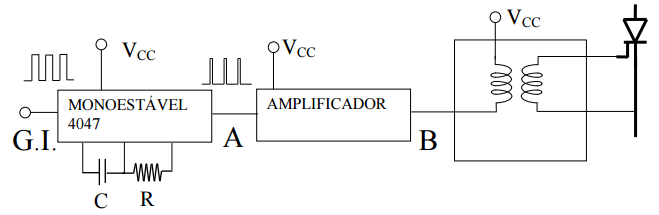
\includegraphics[keepaspectratio=true, scale=0.37]{teoricas/trigger_circuit}
	\caption{Circuito de disparo.}
	\label{fig:circuit_1}
	\vspace{-0.8em}
\end{figure}

O objetivo neste trabalho é assim realizar este circuito com uma frequência de 2 kHz, fazendo para isso uso de um sinal com esta frequência originado por um gerador de impulsos (GI). O circuito de disparo será então composto por uma monoestável que reage ao flanco ascendente do sinal originado pelo GI; tem-se assim à saída da monoestável um impulso cuja duração será função da resistência $R$ e condensador $C$. 

A duração deste impulso deve ser definida consoante as características da \textit{gate} do tiristor que se está a utilizar, sendo neste caso de 10 $\mu$s. Este impulso tem, no entanto, que ser amplificado para que seja injetada corrente suficiente na \textit{gate} do tiristor. Usa-se assim um transístor de ganho elevado, transitando da saturação ao corte, estabelecendo uma tensão no primário do transformador, sempre que surja o impulso na saída da monoestável. As formas de onda destes impulsos podem ser observadas na \autoref{fig:circuit_2}.

\begin{figure}[h]
	\centering
	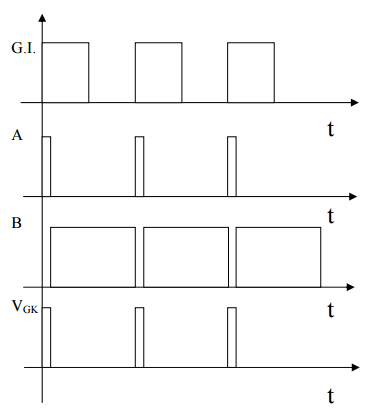
\includegraphics[keepaspectratio=true, scale=0.45]{teoricas/trigger_waveform}
	\caption{Formas de onda das tensões no circuito de disparo.}
	\label{fig:circuit_2}
	\vspace{-0.8em}
\end{figure}

O transformador serve também para que se obtenha o isolamento galvânico entre os circuitos de disparo e de potência.

\subsection{Montagem e equipamento}

A montagem presente na placa impressa utilizada no laboratório pode ser observada na \autoref{fig:circuit_3}.

\begin{figure}[h]
	\centering
	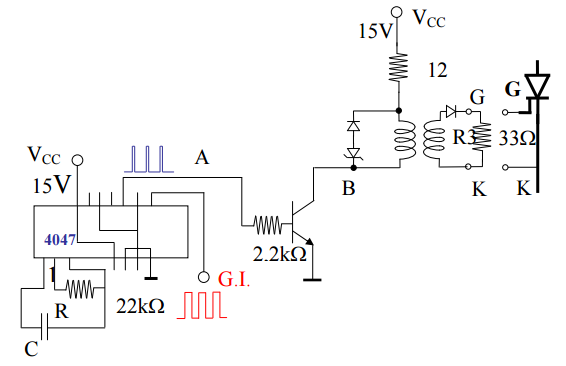
\includegraphics[keepaspectratio=true, scale=0.45]{teoricas/assembly_circuit}
	\caption{Esquema elétrico do circuito de disparo presente na placa impressa.}
	\label{fig:circuit_3}
	\vspace{-0.8em}
\end{figure}

Tal como dito na secção acima, a duração do impulso, $T$, será definida pela resistência $R$ e o condensador $C$ segundo a seguinte fórmula dada pelo fabricante.

\vspace{-3mm}
\begin{equation}
T = 2.88 \ RC.
\end{equation}

Para que se tenha 10 $\mu$s faz-se assim uso de uma resistência com $10$ k$\Omega$ e $0.4$ nF, sem necessidade de uma grande precisão nos valores, pois a exatidão do tempo de disparo neste circuito não é prevalente.

O equipamento a utilizar na condução do trabalho é assim:

\vspace{-2mm}

\begin{itemize}
	\item 1 osciloscópio;
	\vspace{-2mm}	
	\item 1 sonda de corrente;
	\vspace{-2mm}	
	\item 1 gerador de impulsos;
	\vspace{-2mm}	
	\item 2 fontes de alimentação;
	\vspace{-2mm}	
	\item 2 multímetros;
	\vspace{-2mm}	
	\item 1 placa de circuito impresso.
\end{itemize}

\pagebreak

\section{Condução do Trabalho}

\subsection{Estudo do circuito de disparo}

Em primeira instância apenas se realizam as ligações do circuito de disparo à fonte de alimentação. Após as ligações feitas sintoniza-se o GI para que se obtenha na saída uma onda retangular de amplitude $0$ a $15$ a uma frequência de $2$ kHz.

\subsubsection{Formas de onda da tensão entre o ponto A e a massa e entre o ponto B e a massa}

Feito isto, podem observar-se as formas de onda entre o ponto A e a massa e o ponto B e a massa no osciloscópio tal como na \autoref{fig:photo 1}.

\begin{figure}[h]
	\centering
	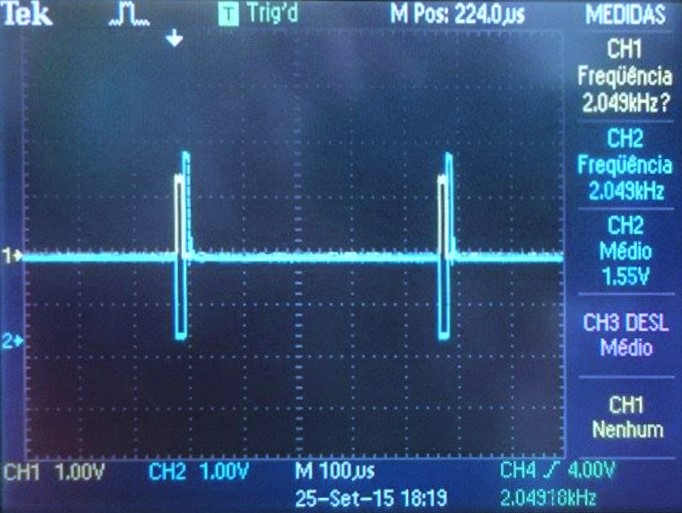
\includegraphics[keepaspectratio=true, scale=0.55]{img/fig4}
	\caption{Tensões nos pontos A (a amarelo) e B (a azul).}
	\label{fig:photo 1}
	\vspace{-0.8em}
\end{figure}

Tem-se assim no canal $1$ (amarelo) a tensão no ponto A e no canal $2$ (azul) a tensão no ponto B. Para o canal 1 observa-se uma onda quadrada compreendida entre 0 e 14,8 V, frequência de $2$ kHz, duração de impulso de $13$ $\mu$s e um fator de ciclo de 2,6\%. O canal $2$ apresenta uma onda retangular com $1,5$ V no qual existe um pico de tensão no flanco ascendente com $3,4$ V estabilizando ao fim de aproximadamente $15$ $\mu$s. A duração do sinal retangular no canal 2 é de aproximadamente 470 $\mu$s o que leva a um fator de ciclo de 94\%.

Na \autoref{fig:photo 2} fez-se \textit{zoom} de forma a que o pico de tensão da onda retangular no canal 2 se possa observar melhor, assim como a relação entre as tensões em A e B.

\pagebreak

\begin{figure}[h]
	\centering
	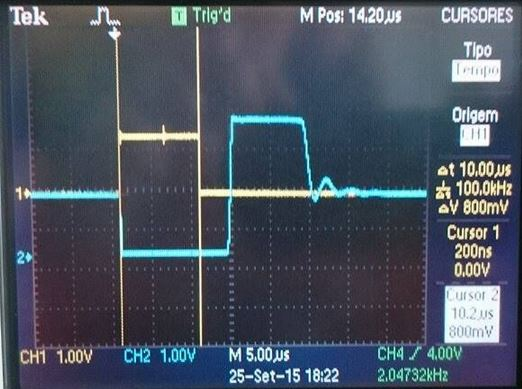
\includegraphics[keepaspectratio=true, scale=0.6]{img/fig5}
	\caption{\textit{Zoom} das tensões nos pontos A e B.}
	\label{fig:photo 2}
	\vspace{-0.8em}
\end{figure}

Este pico deve-se a que, no momento em que o transístor entra em condução, a bobina encontra-se magnetizada ficando os díodos diretamente polarizados, sendo que a tensão em B será a soma entre a tensão no primário do transformador e VCC. Após o período de desmagnetização esta estabiliza no valor devido, VCC. 

Existe também um atraso apreciável entre a tensão em A e B que se deve ao tempo de passagem do transístor da saturação para o corte.

\subsubsection{Díodos no primário do transformador}

Considera-se agora relevante enunciar a funcionalidade dos díodos presentes no circuito. Em primeiro tem-se o díodo ligado ao primário do transformador cuja função é essencialmente garantir a continuidade da corrente quando o transístor passa ao corte, ficando assim a bobina salvaguardada de potenciais descontinuidades na corrente (o que é essencial uma vez que, na bobina, a corrente é variável de estado), garantindo o bom funcionamento do circuito. 

Tem-se ainda o díodo Zenner cujo objetivo é diminuir o tempo de desmagnetização da bobina. Isto é devido à superior tensão imposta por este díodo aos terminais do transformador (tensão de Zenner), elevando assim a corrente que ali circula. A circulação de corrente pelos díodos acontece até que haja a total desmagnetização da
bobina.

\subsubsection{Tensão no primário do transformador em função do díodo Zenner}

A alteração provocada pelo díodo Zenner no comportamento do circuito é evidenciada na \autoref{fig:photo 3} e \autoref{fig:photo 4}.

\pagebreak

\begin{figure}[h]
	\centering
	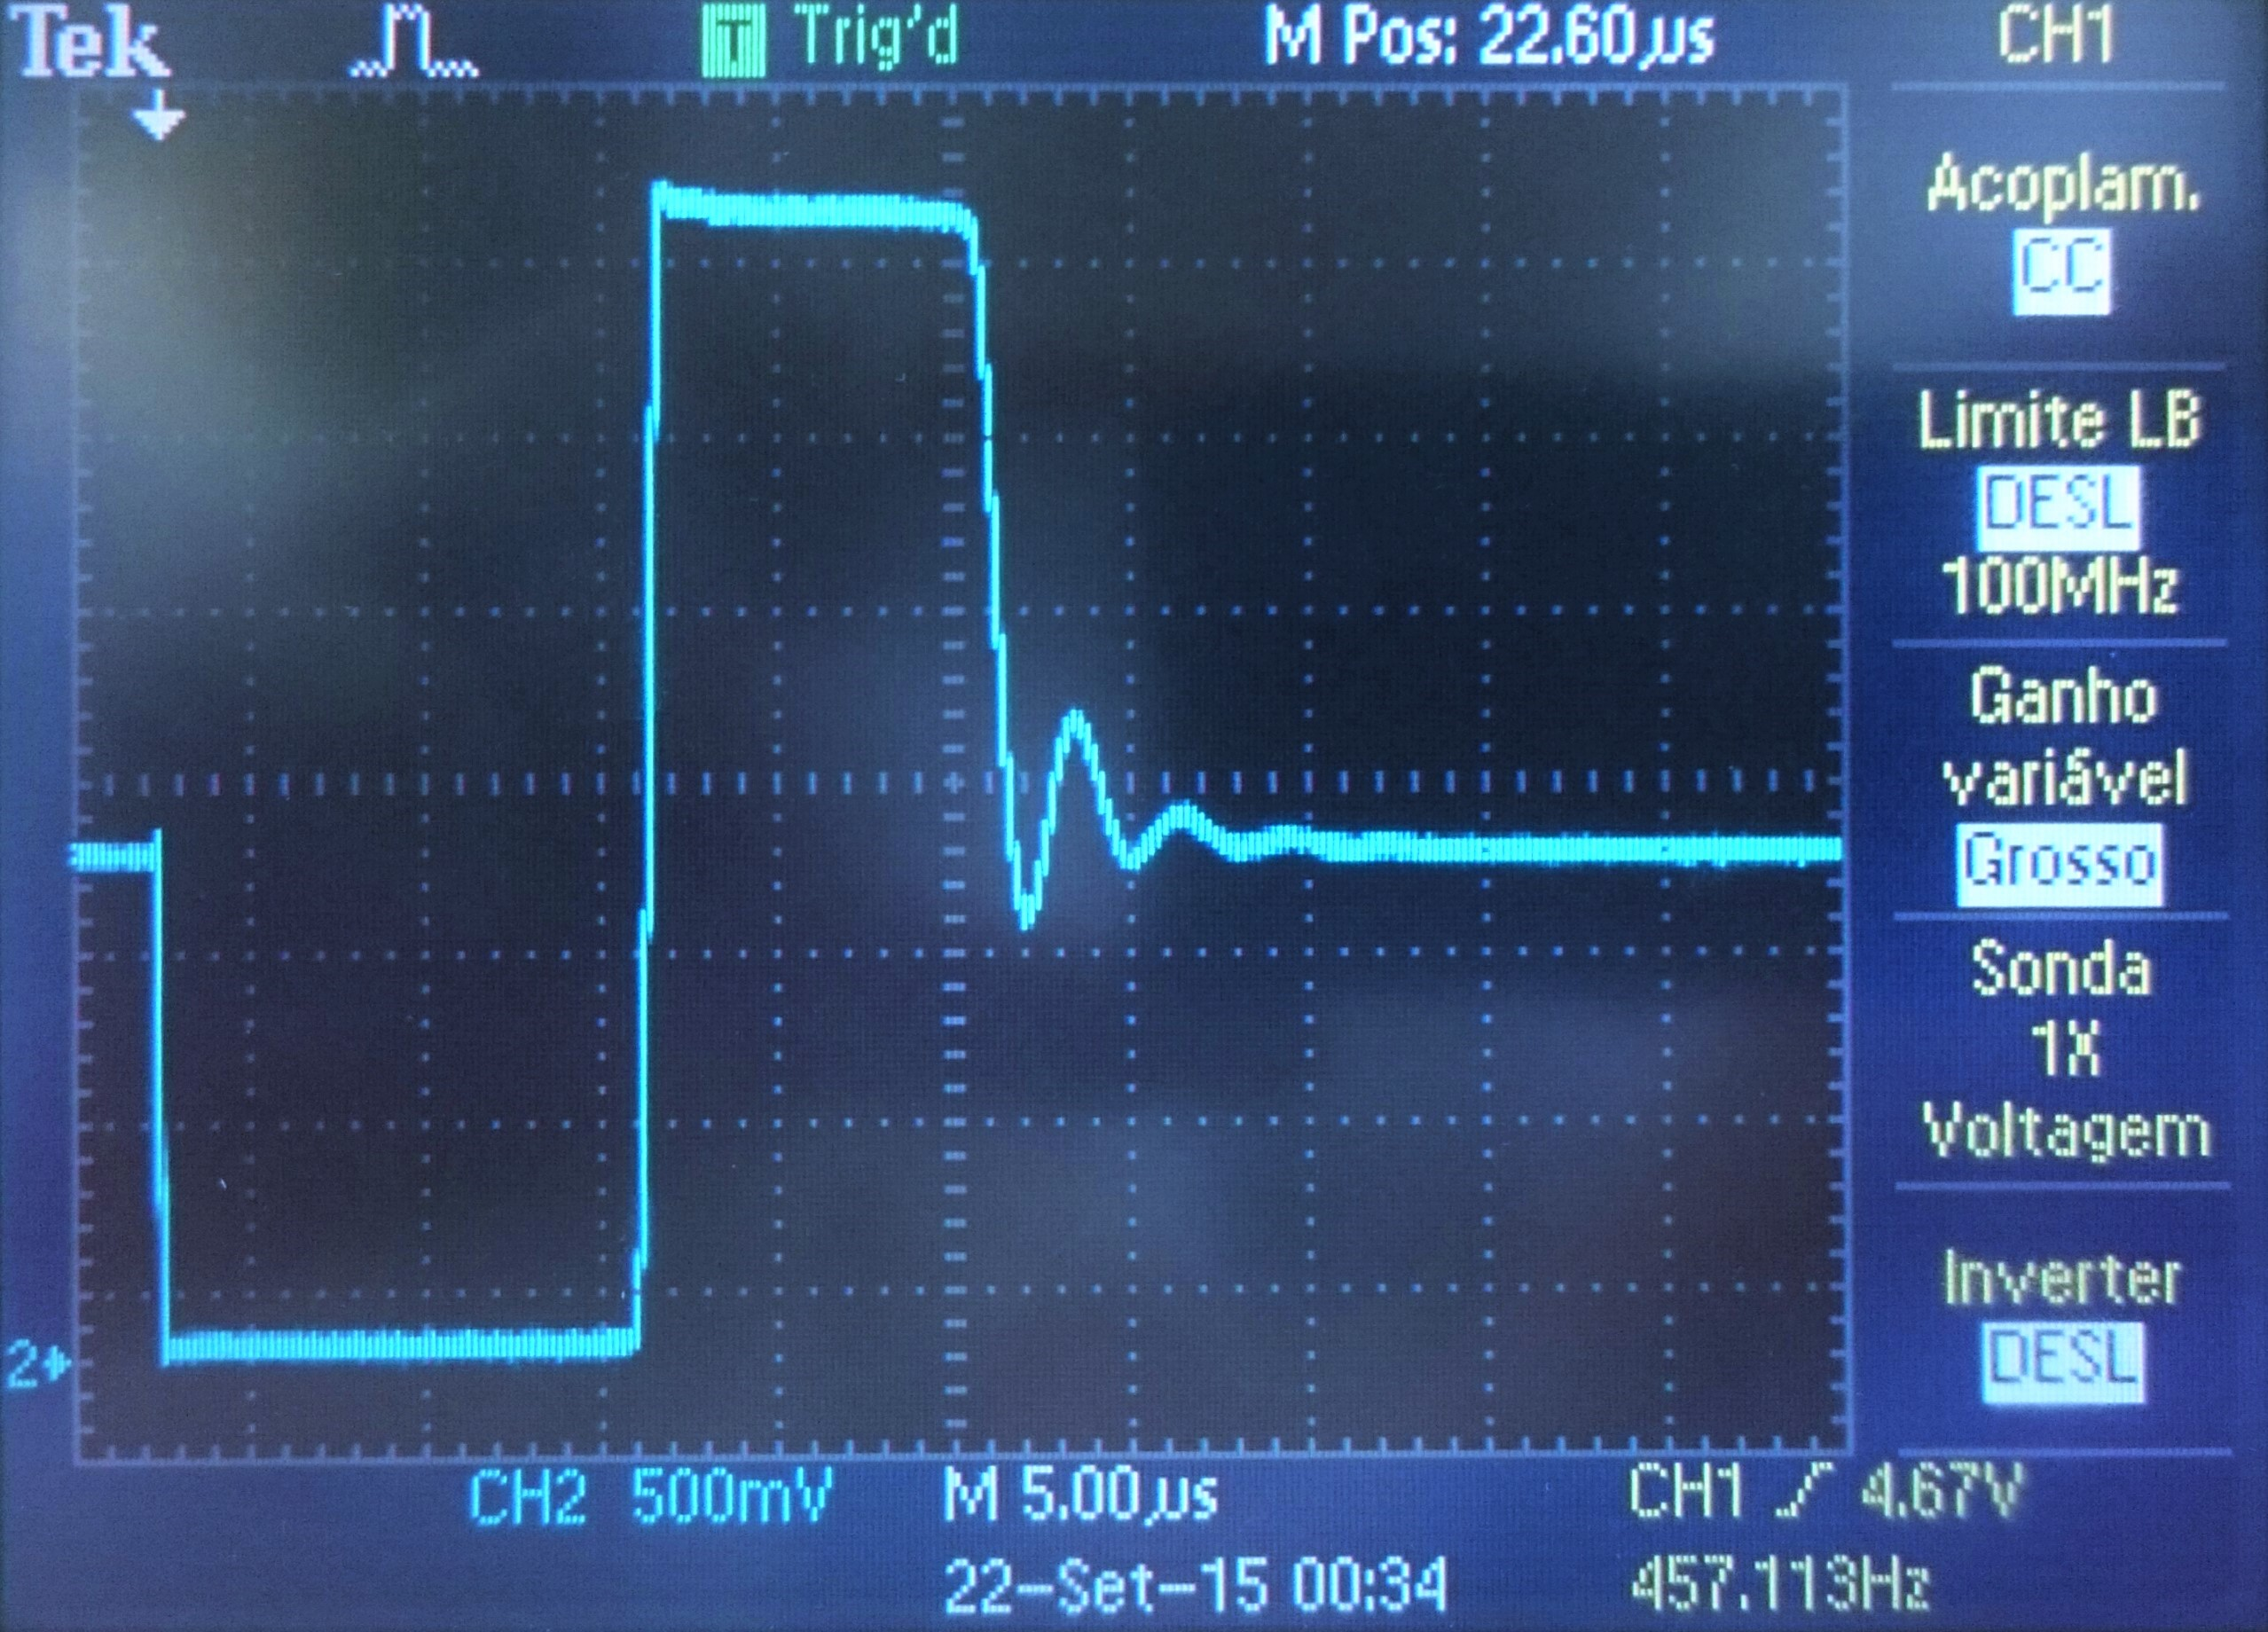
\includegraphics[keepaspectratio=true, scale=0.15]{img/DSC0118}
	\caption{Tensão no ponto B com o díodo Zenner.}
	\label{fig:photo 3}
	\vspace{-0.8em}
\end{figure}

\begin{figure}[h]
	\vspace{3mm}
	\centering
	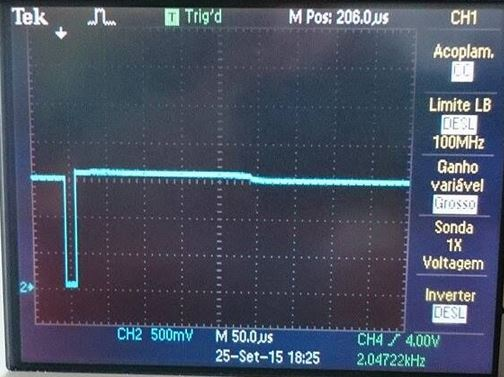
\includegraphics[keepaspectratio=true, scale=0.63]{img/fig7}
	\caption{Tensão no ponto B sem o díodo Zenner.}
	\label{fig:photo 4}
	\vspace{-0.8em}
\end{figure}

Na \autoref{fig:photo 3} pode concluir-se que o tempo de desmagnetização é relativamente curto, cerca de $30$ $\mu$s em oposição ao tempo de desmagnetização observável na \autoref{fig:photo 4}, onde será aproximadamente $225$ $\mu$s, valor muito superior ao caso em que se faz uso do díodo Zenner.

O díodo Zenner conduz quando inversamente polarizado (neste caso, a tensão de Zenner é de $-17$ V), o que leva a uma dissipação muito mais rápida, e consequentemente acelera o processo de desmagnetização. Verifica-se que, em ambos os casos, a área da curva de magnetização é idêntica à área da curva de desmagnetização. Sem díodo Zenner, o valor da curva de desmagnetização é mais baixo, pelo que leva mais tempo a satisfazer este requisito. 

\subsubsection{Tensão entre a \textit{gate} e o cátodo do tiristor}

Seguidamente visualizou-se a tensão aos terminais da resistência R\textsubscript{3},  V\textsubscript{GK} tal como se tem na \autoref{fig:photo 5}.

\begin{figure}[h]
	\centering
	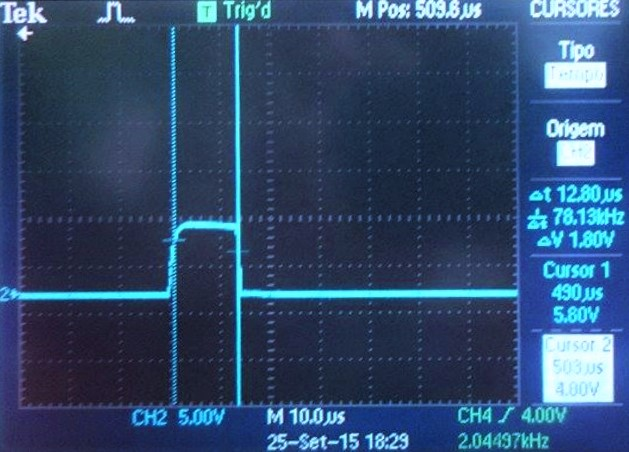
\includegraphics[keepaspectratio=true, scale=0.63]{img/fig8}
	\caption{Tensão V\textsubscript{GK} na resistência R\textsubscript{3}.}
	\label{fig:photo 5}
	\vspace{-0.8em}
\end{figure}

Trata-se portanto de um sinal retangular com duração de impulso de 13 $\mu$s, amplitude de aproximadamente 8 V e um fator de ciclo de 2,6\% que são as características necessárias para se ter o sinal de comando do tiristor.

De forma a que a primeira parte do trabalho esteja concluída passou-se a desligar os terminais da resistência, seguido da realização das ligação dos pontos G e K à \textit{gate} e cátodo do tiristor, respetivamente.

\subsection{Estudo do circuito de potência}

Pretende-se agora verificar, como já foi referido, que o tiristor é um dispositivo que, por si só, não tem a capacidade de cortar a corrente que conduz. Assim, efetuam-se duas montagens distintas, tal como se tem na \autoref{fig:teorica1}.

\begin{figure}[H]
	\centering
	\subfloat[]{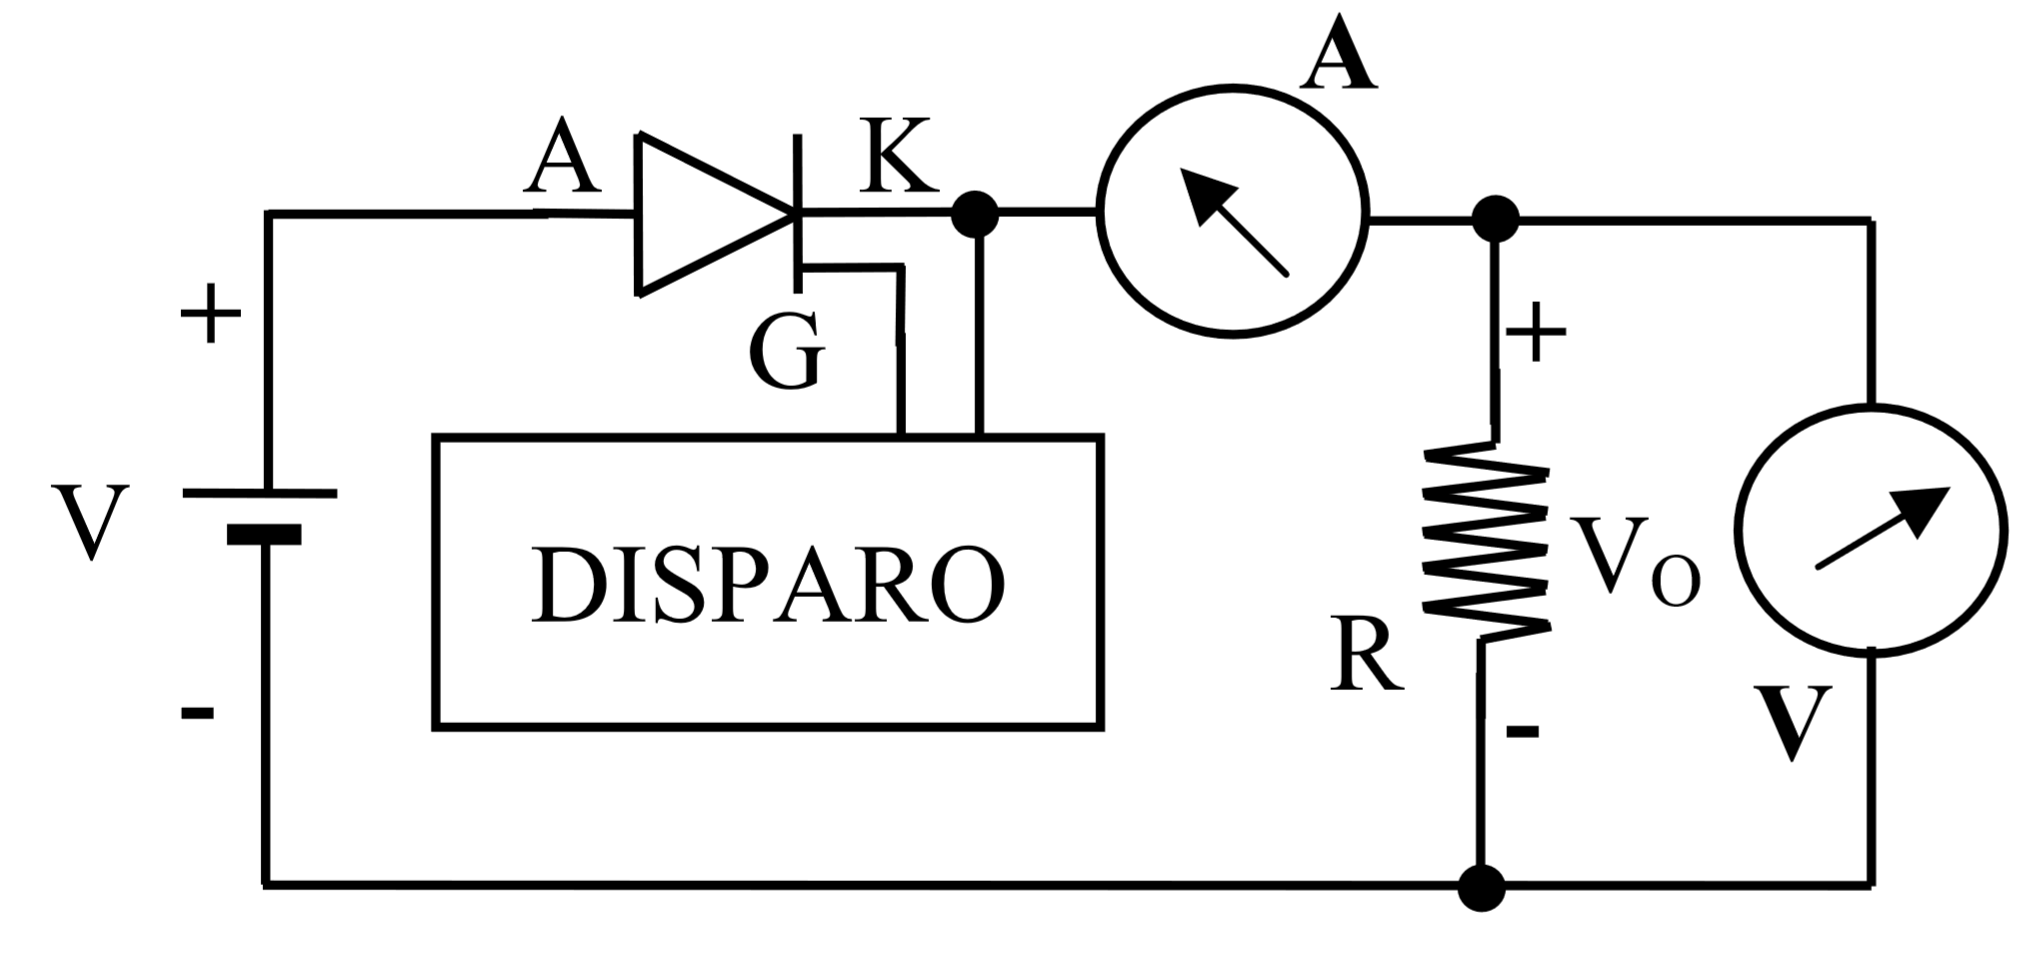
\includegraphics[keepaspectratio=true, scale=0.17]{teoricas/no_cut}}
	\hspace{8mm}
	\subfloat[]{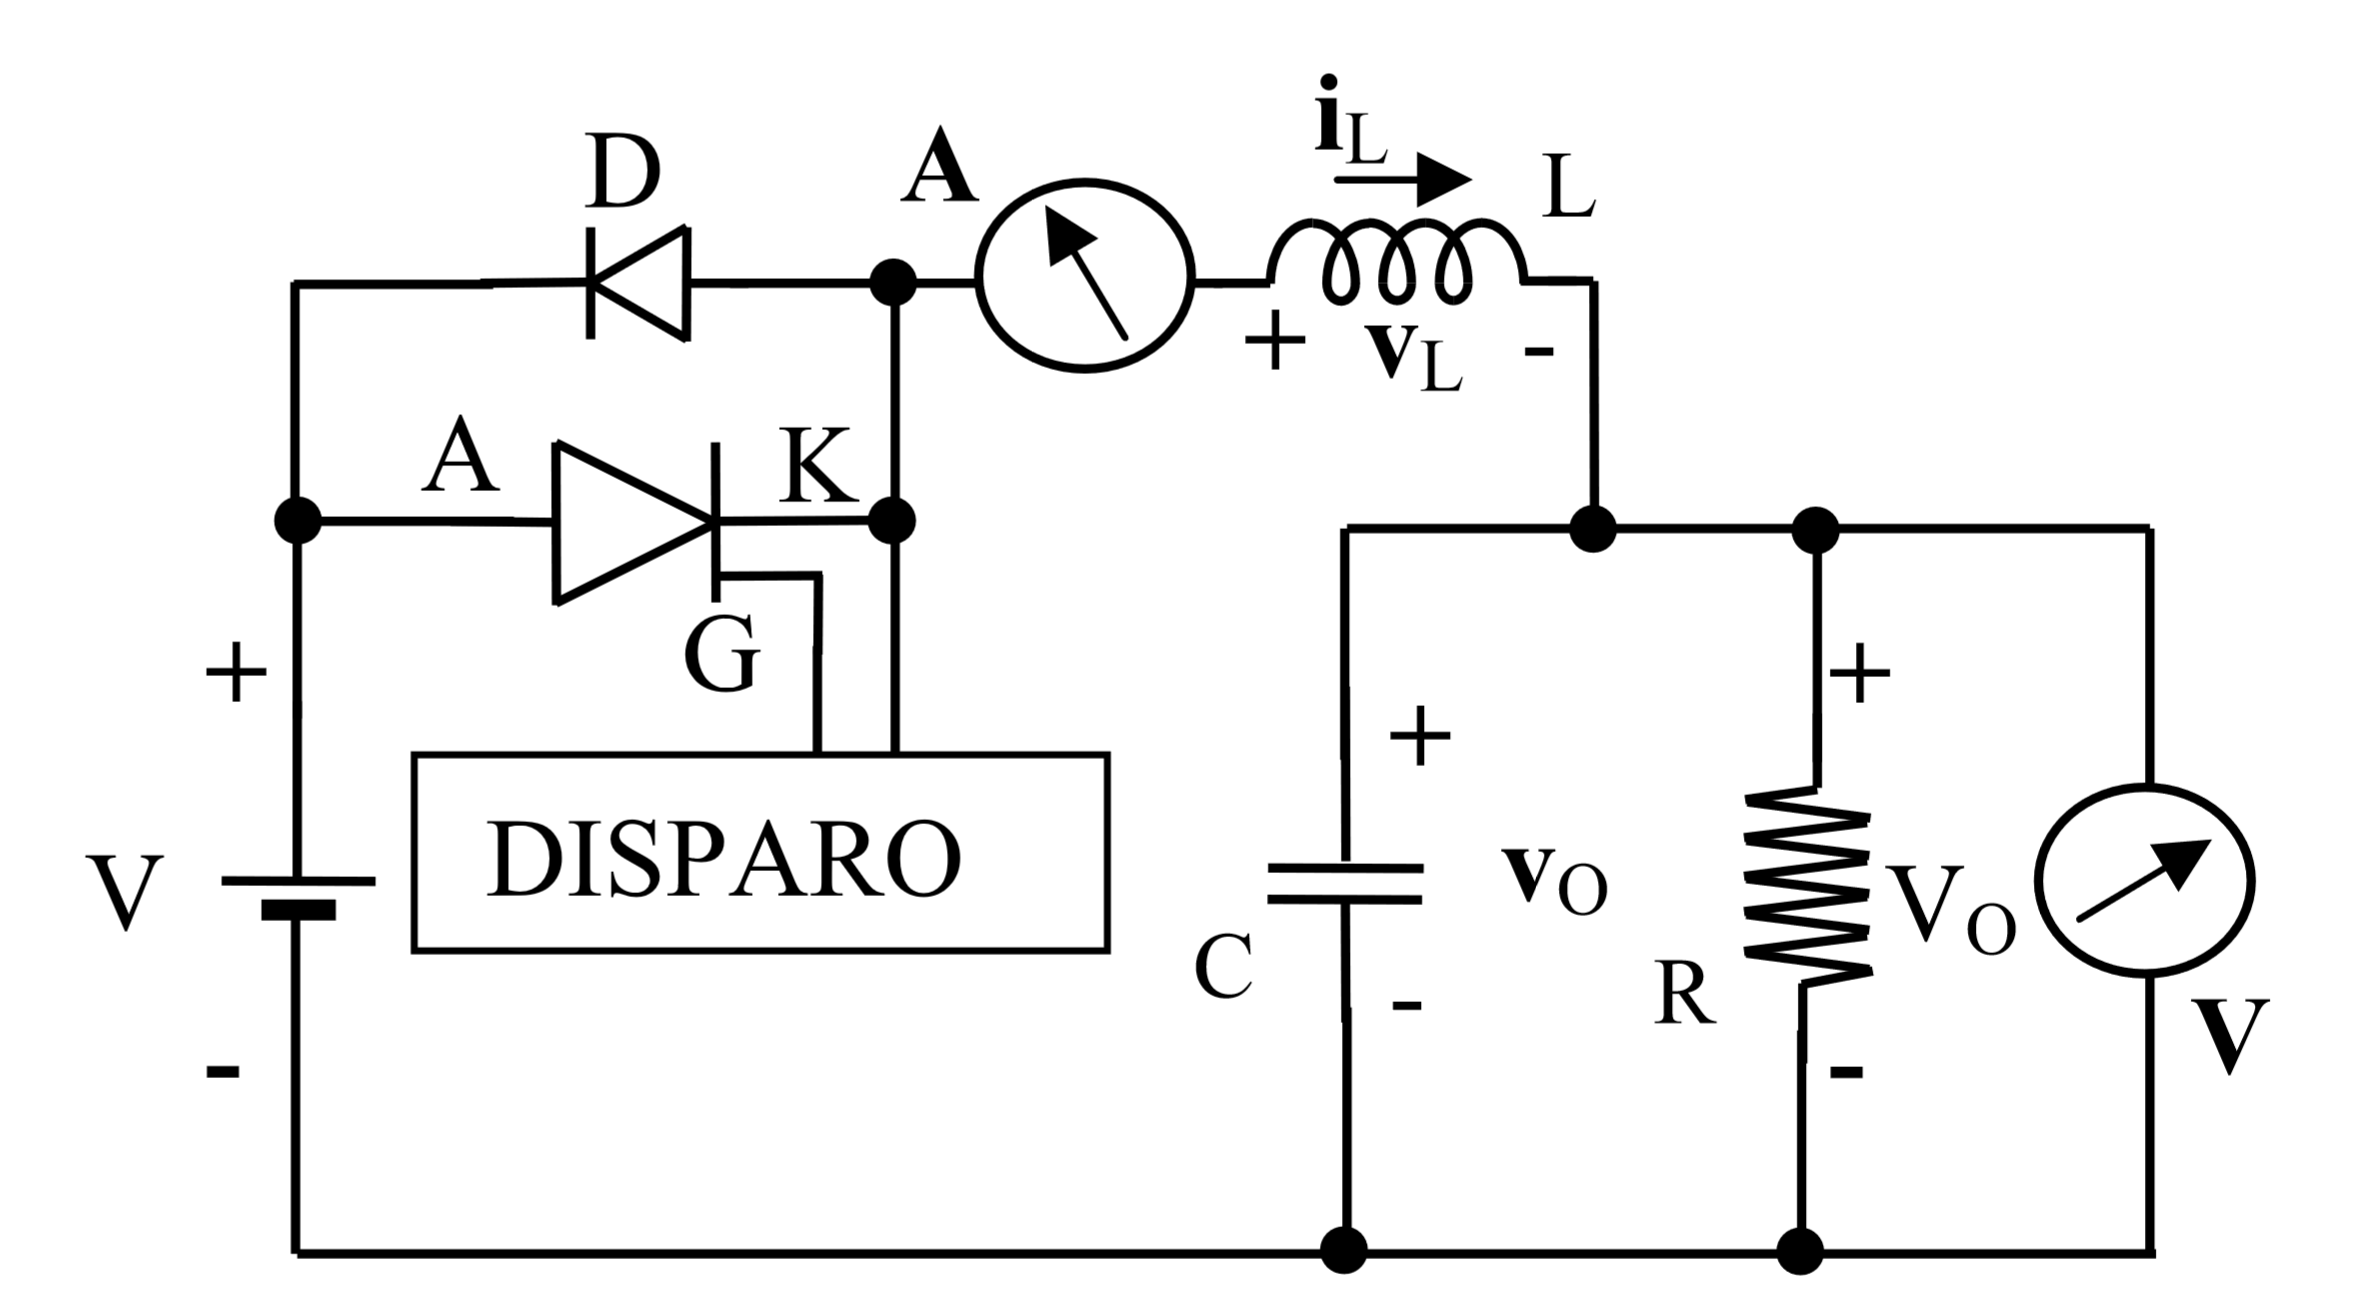
\includegraphics[keepaspectratio=true, scale=0.17]{teoricas/yes_cut}}
	\caption{Circuito de potência sem comutação do tiristor (a) e circuito de potência com comutação do tiristor por ação da carga (b).}
	\label{fig:teorica1}
	\vspace{-0.8em}
\end{figure}

No circuito da \autoref{fig:teorica1}(a), o tiristor depois de disparado não volta a passar ao corte, mesmo depois de retirado o impulso de \textit{gate}. Já no circuito da \autoref{fig:teorica1}(b) o tiristor comuta por ação da carga.

\subsubsection{Valores do voltímetro e amperímetro}

Efetuada a montagem da \autoref{fig:teorica1}(a) leram-se os valores (DC) indicados no voltímetro e amperímetro.

Regulada a fonte de alimentação para 20 V e descontando a queda de 1 V no tiristor, o valor registado na carga será de 19 V. A resistência na carga tem um valor 100 $\Omega$ e assim, de acordo com a lei de Ohm, tem-se uma corrente de 190 mA.

\subsubsection{Variações da corrente e tensão na carga em função do GI}

Verifica-se atuando no GI (em amplitude, frequência ou fator de ciclo) que não existem alterações na corrente e tensão na carga. O circuito apresentado na \autoref{fig:teorica1}(a) tem uma carga puramente resistiva e, como tal, uma vez que o tiristor começa a conduzir já não volta ao corte por variações causadas no GI.

Assim se percebe como o tiristor, uma vez que seja disparado, e tenha uma corrente de ânodo maior que a corrente de manutenção (conceito a explorar futuramente) continua a conduzir devido à realimentação positiva, mesmo que o sinal proveniente do GI seja removido. 


\subsubsection{Corrente de lançamento e corrente de manutenção}

Variando a tensão de alimentação do circuito de potência, e consequentemente a corrente na carga, determinou-se a corrente de lançamento e a corrente de manutenção.

\hspace{30mm} I\textsubscript{lançamento} = 120 mA \hspace{5mm} I\textsubscript{manutenção} = 90 mA 

A corrente de lançamento ($i_L$) corresponde à mínima corrente de ânodo necessária para manter o tiristor no estado de condução imediatamente após este ter sido disparado. Assim, uma vez que o dispositivo tenha sido ligado pelo terminal da \textit{gate} manter-se-á nesse \textit{on-state} desde que a corrente de ânodo seja maior que $i_L$.

Desde que o ânodo se mantenha polarizado positivamente, o tiristor não pode ser desligado até que a corrente de ânodo seja menor que a corrente de manutenção ($i_H$). Assim, se a corrente de ânodo for reduzida abaixo de $i_H$ o tiristor entra no estado de bloqueio, pois essa é a mínima corrente para manter o tiristor no estado de condução.

A corrente de lançamento é maior que a corrente de manutenção.

Na \autoref{fig:caracteristica} pode-se ver a característica $V\textsubscript{AK}(I)$ do tiristor, onde melhor se compreende os conceitos de corrente de lançamento e manutenção.

\pagebreak

\begin{figure}[h]
	\centering
	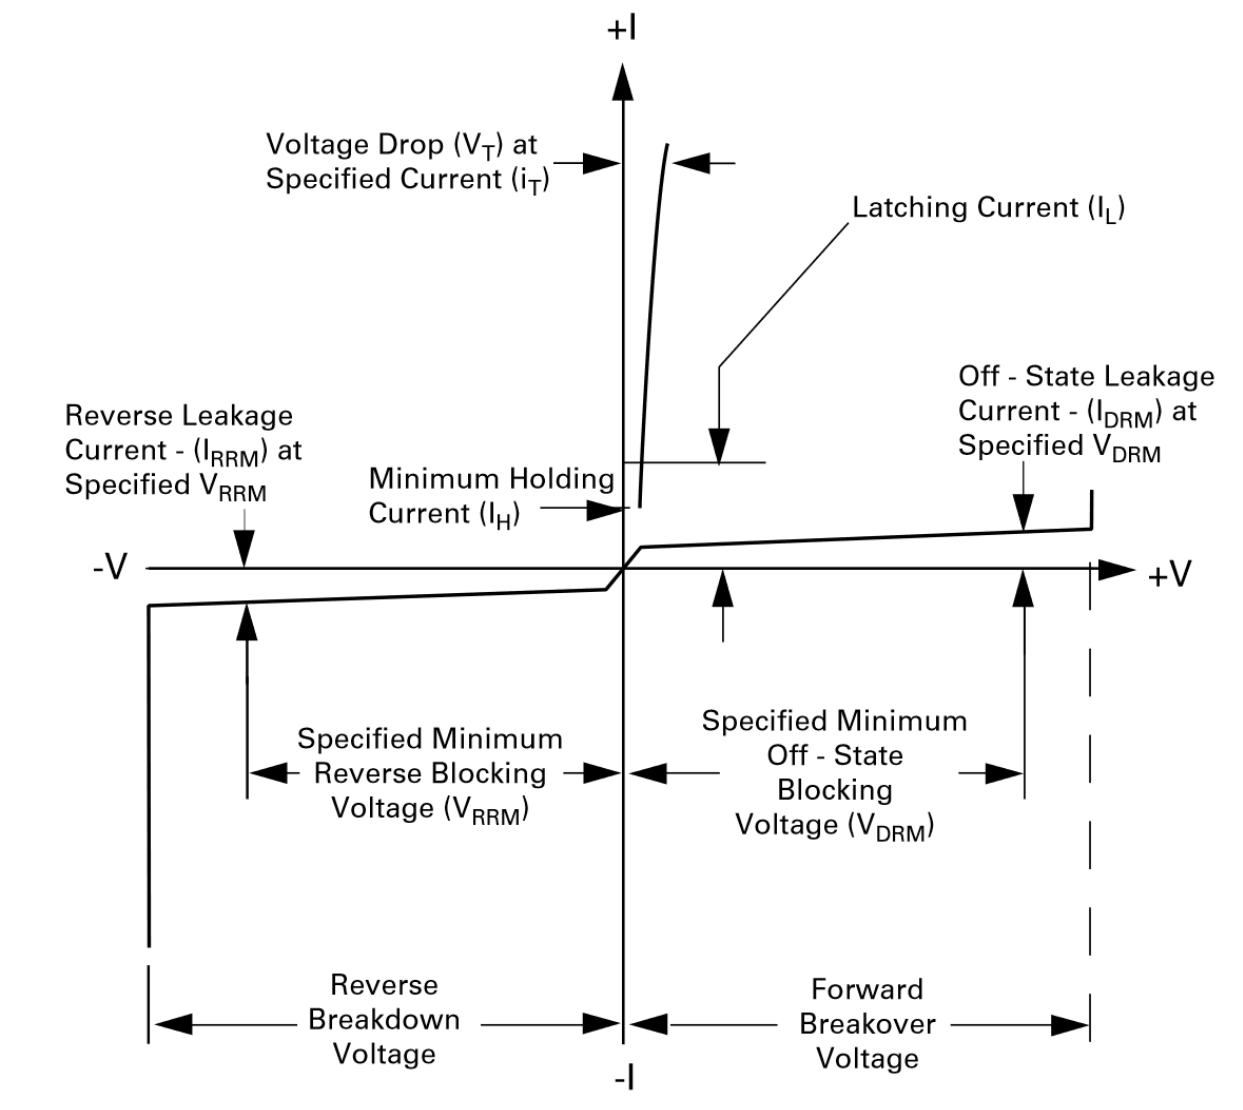
\includegraphics[keepaspectratio=true, scale=0.33]{teoricas/caracteristica}
	\caption{Característica $v(i)$ do tiristor.}
	\label{fig:caracteristica}
	\vspace{-0.8em}
\end{figure}

\subsubsection{Formas de onda da tensão no condensador e da corrente na bobine}

Nesta fase do trabalho efetua-se a montagem da \autoref{fig:teorica1}(b), colocando-se em antiparalelo com o tiristor o díodo rápido. 

A forma dos sinais de tensão no condensador e corrente na bobine podem ser observadas na \autoref{fig:imagem1}.

\begin{figure}[h]
	\centering
	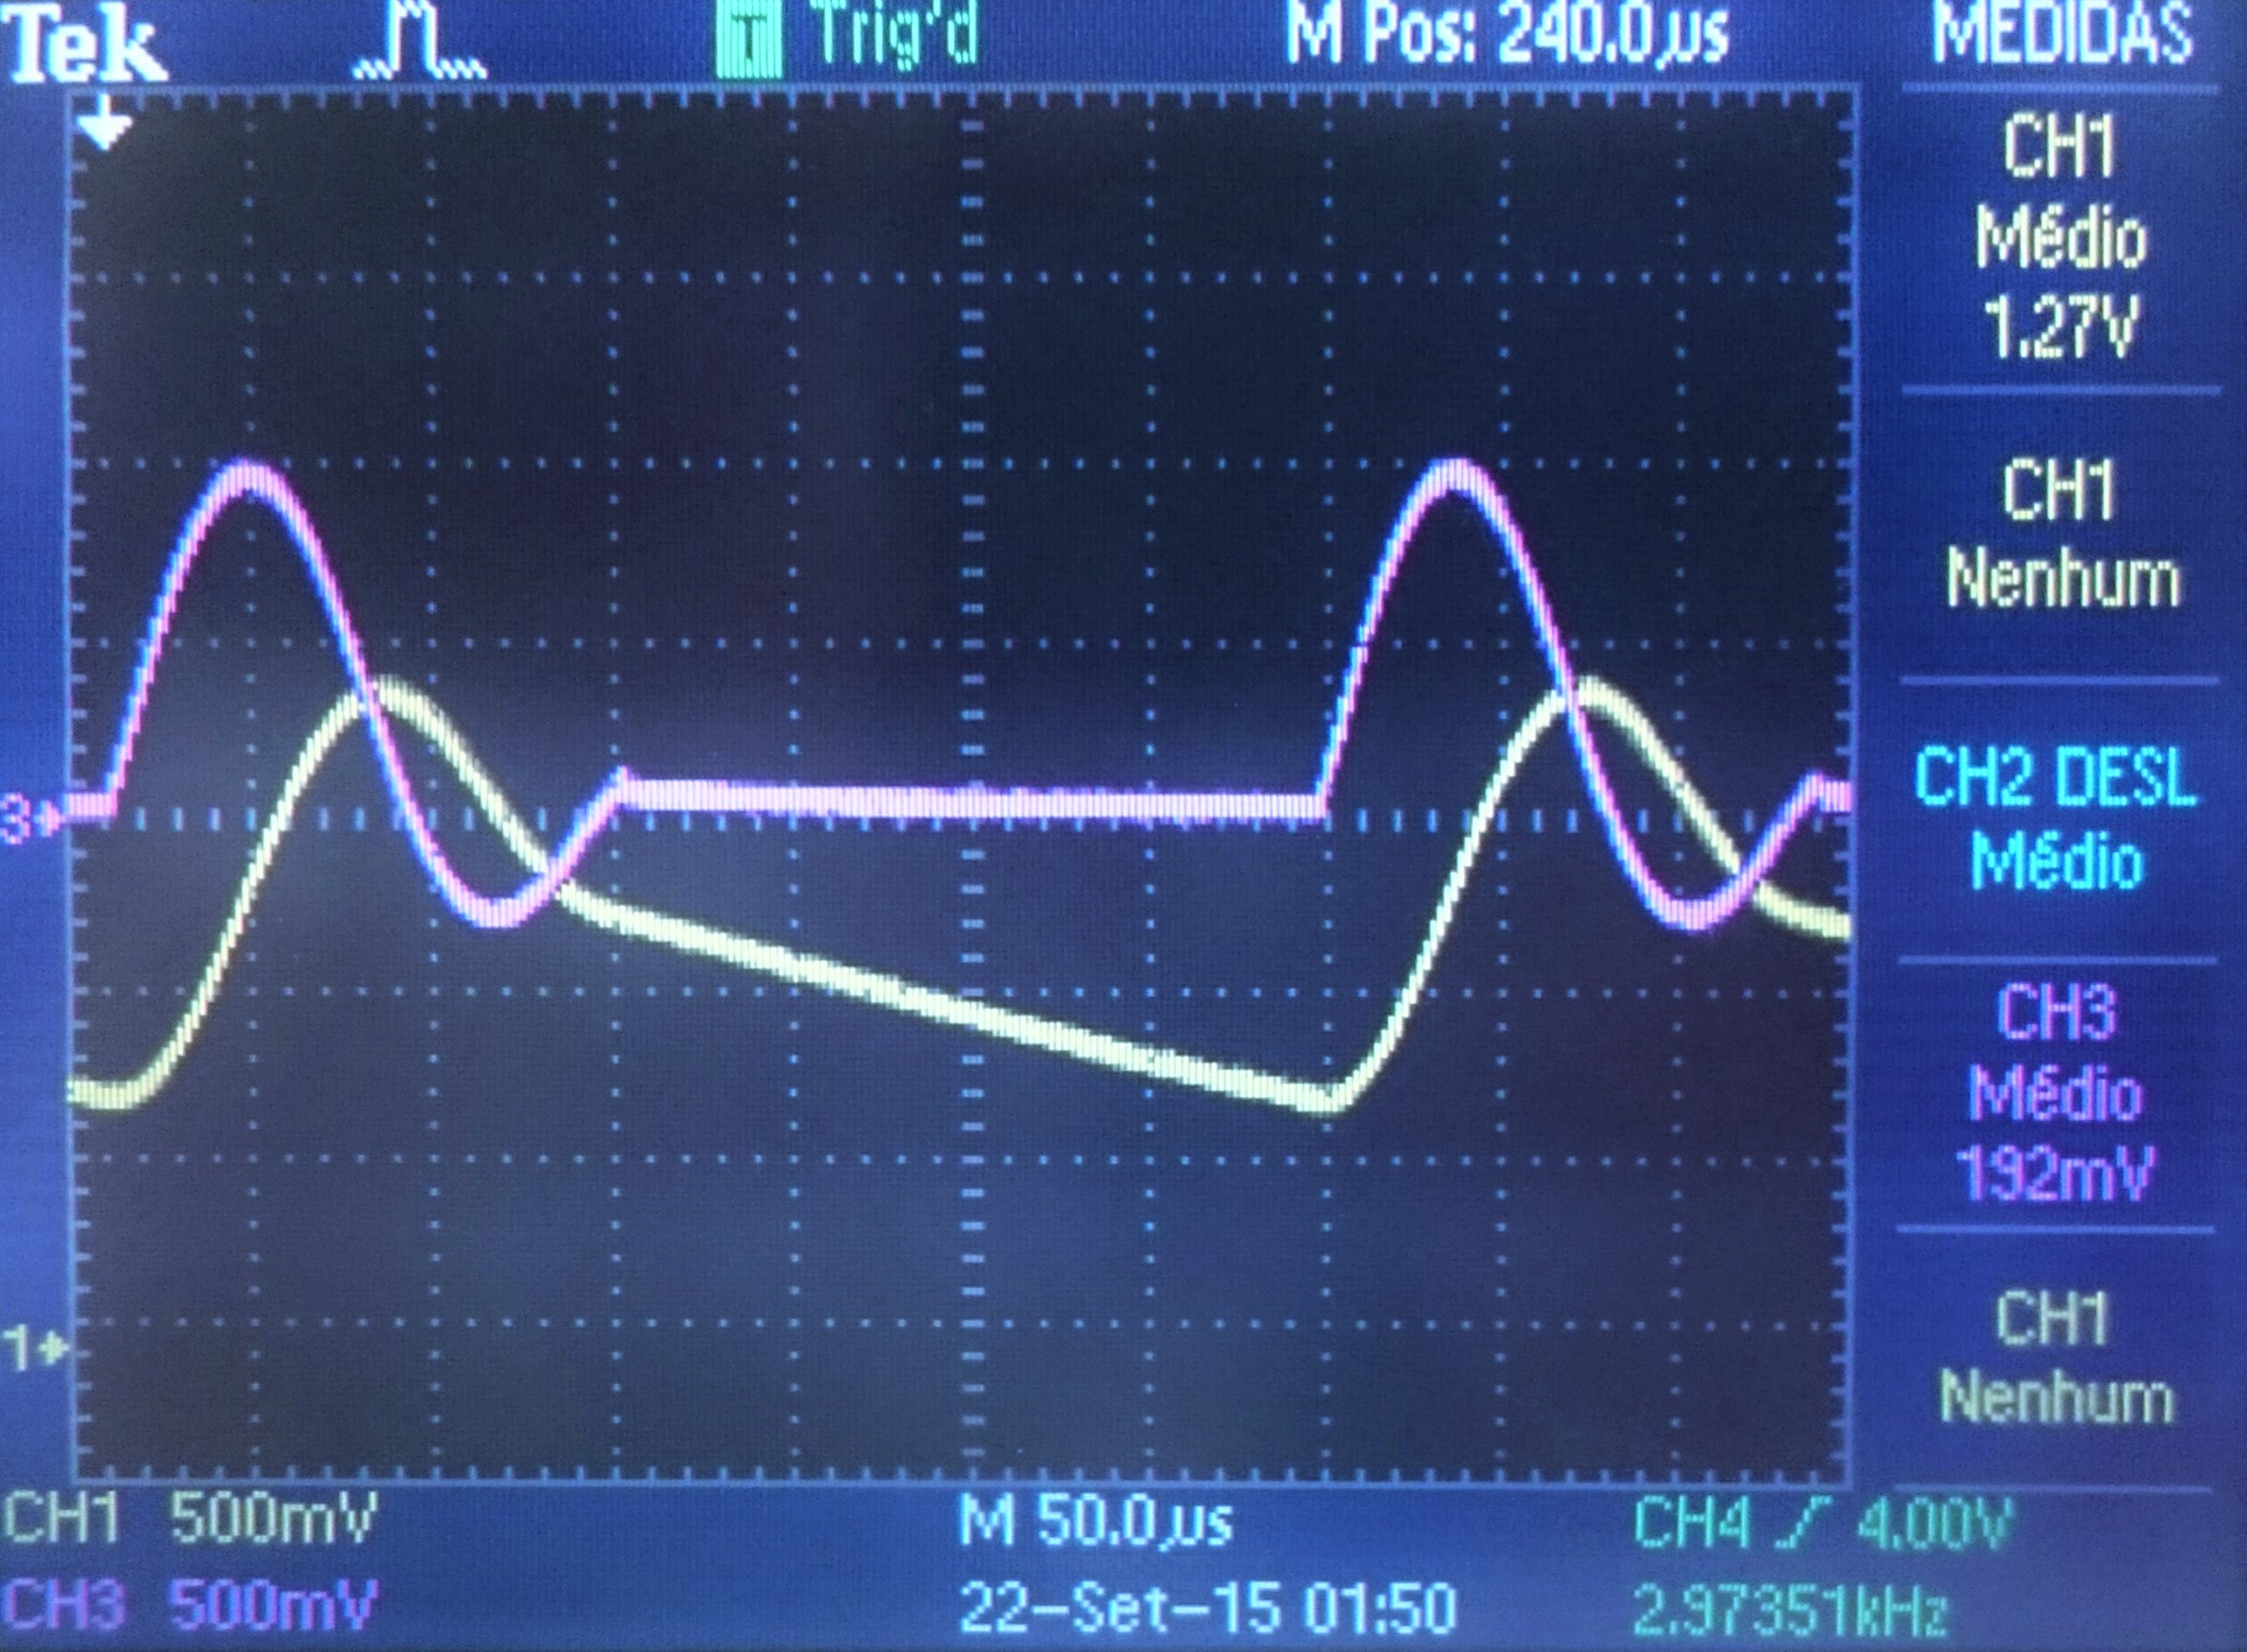
\includegraphics[keepaspectratio=true, scale=0.17]{img/imagem1}
	\caption{Tensão no condensador (a amarelo) e corrente na bobine (a rosa).}
	\label{fig:imagem1}
	\vspace{-0.8em}
\end{figure}

Como se pode verificar, no período de condução a corrente e a tensão apresentam forma sinusoidal (sinusoidal amortecida no caso da corrente). No período de corte a corrente na bobine é nula e a tensão no condensador decresce de forma exponencial, o que corresponde à sua descarga devido à resistência de carga que se encontra em paralelo com o condensador.

Também na \autoref{fig:imagem1} se pode verificar o comportamento oscilatório do circuito.

\subsubsection{Formas de onda da tensão e corrente no díodo rápido em antiparalelo}

A forma dos sinais de corrente e tensão no díodo em antiparalelo podem ser observadas na \autoref{fig:imagem2}.

\begin{figure}[h]
	\centering
	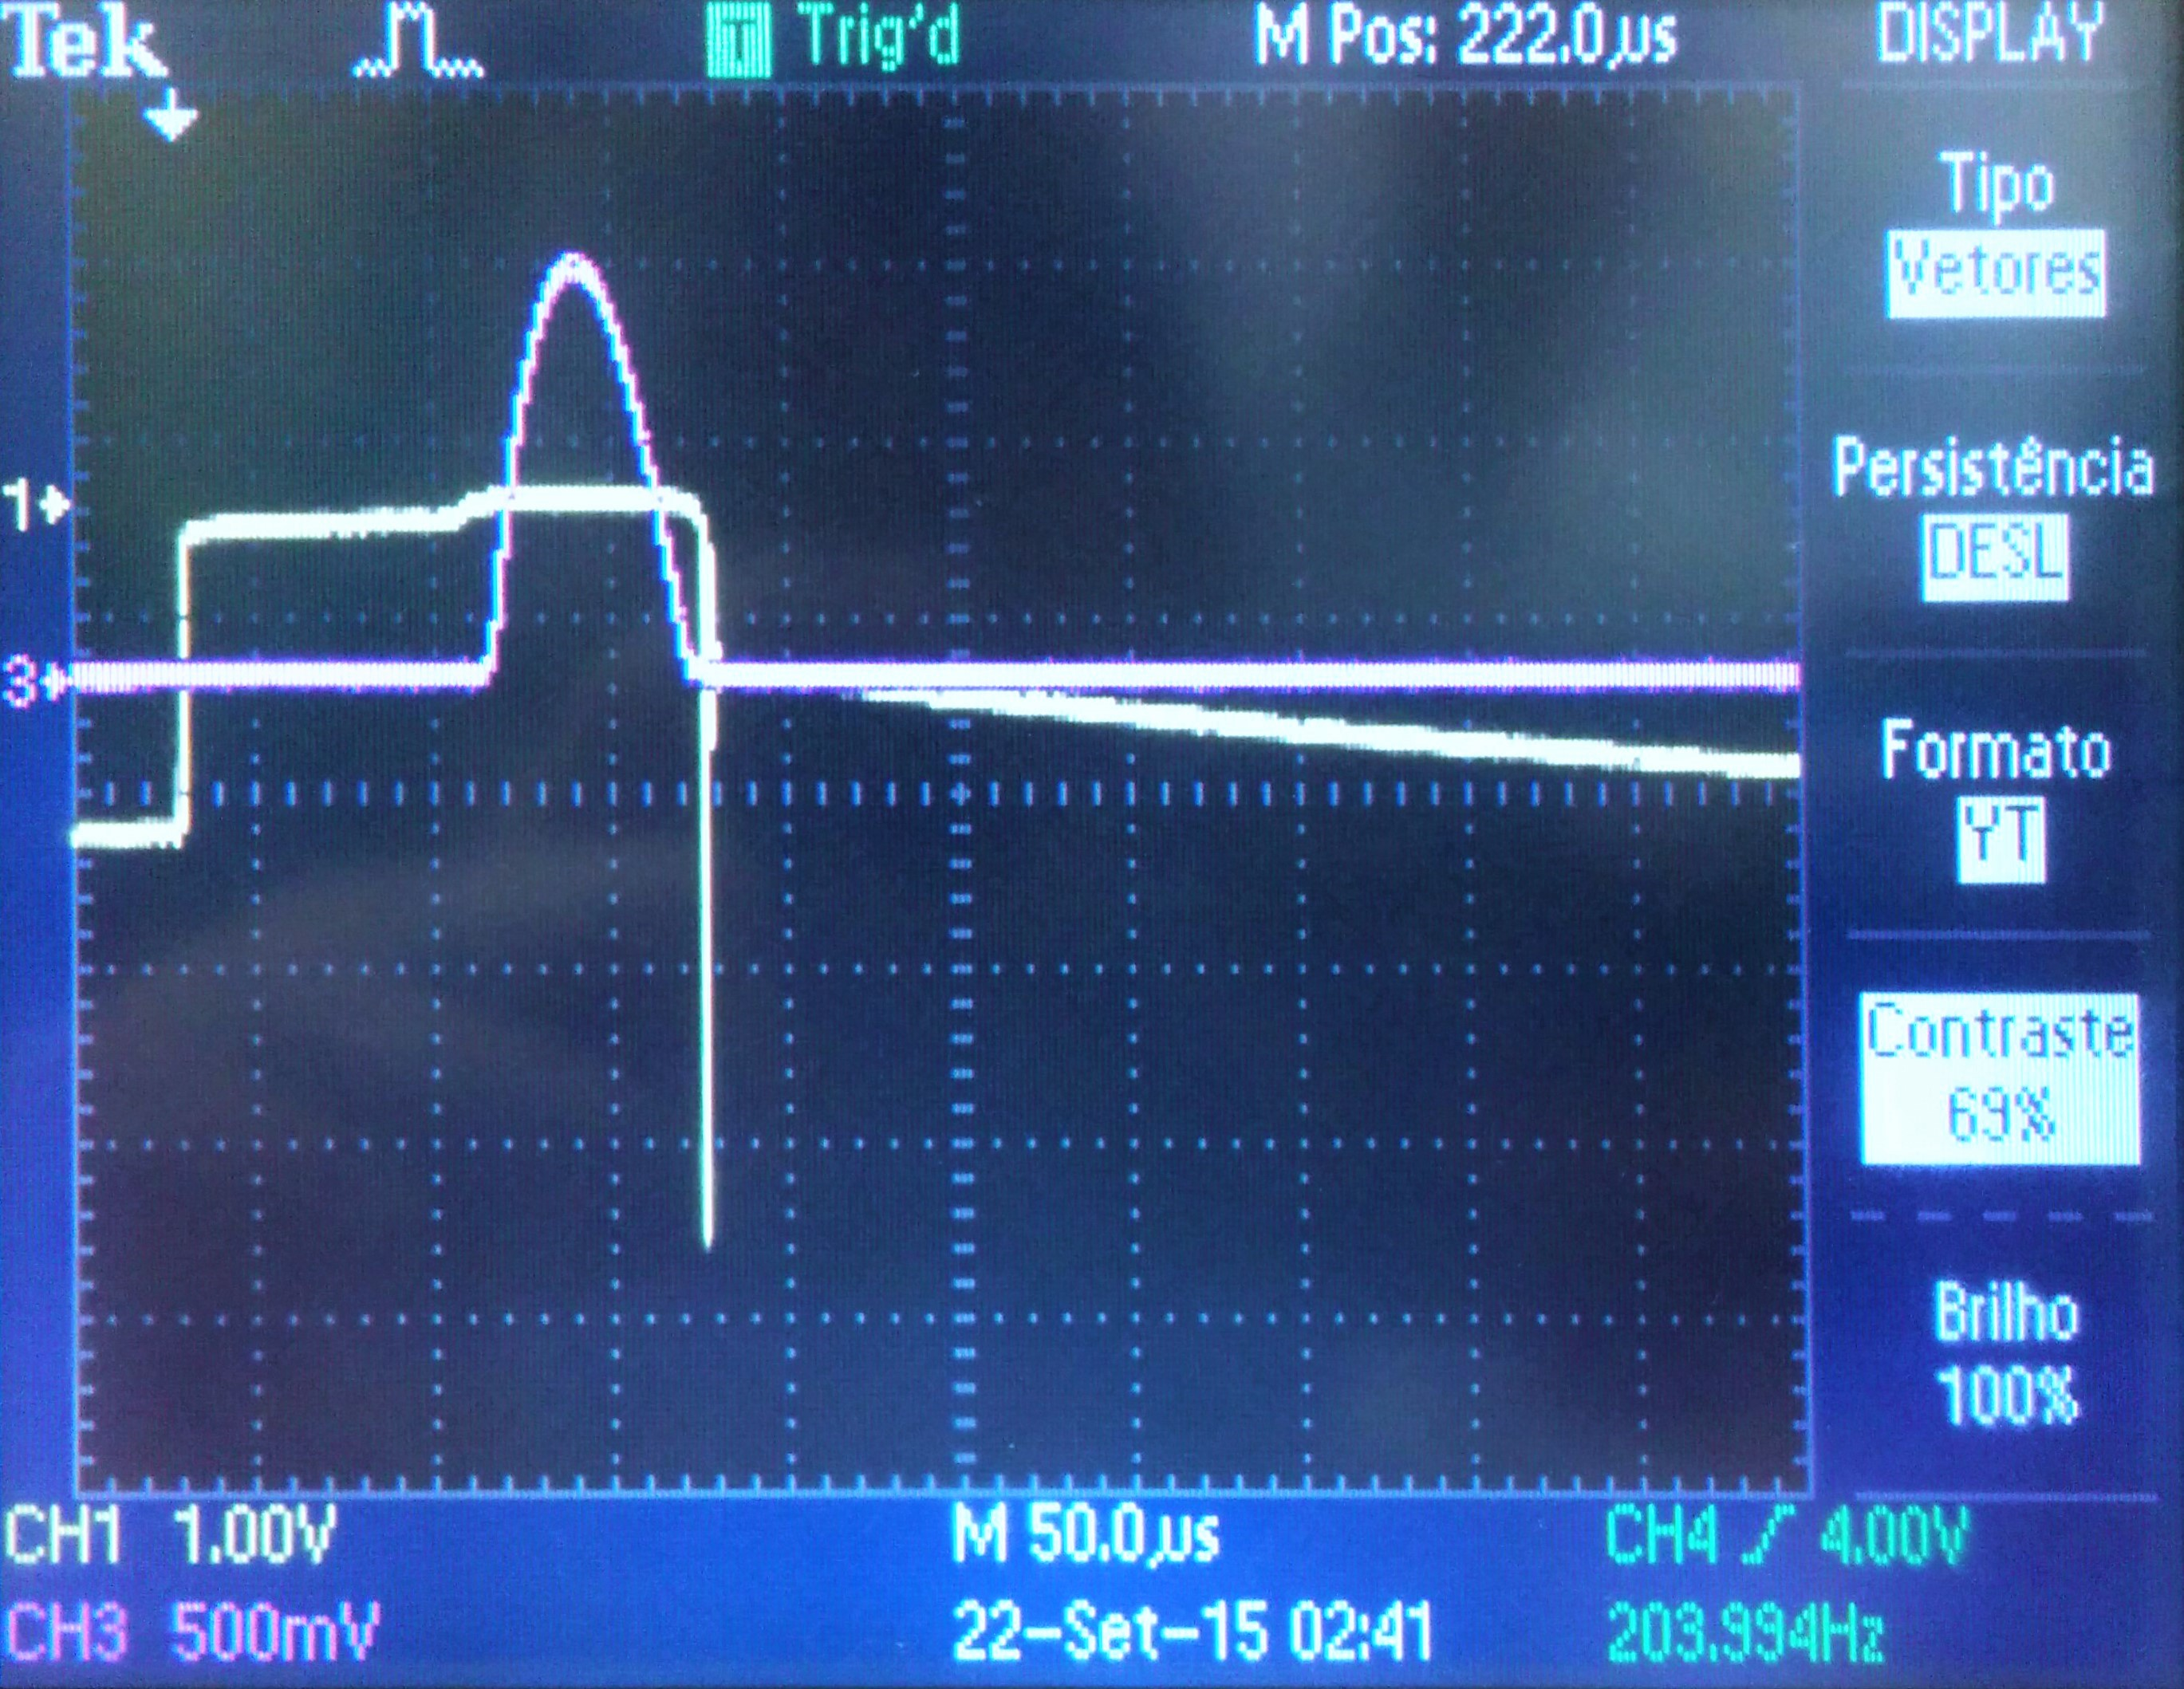
\includegraphics[keepaspectratio=true, scale=0.12]{img/imagem2}
	\caption{Tensão (a amarelo) e corrente (a rosa) no díodo rápido.}
	\label{fig:imagem2}
	\vspace{-0.8em}
\end{figure}

Nos períodos em que o tiristor conduz tem-se uma forma sinusoidal na corrente, que corresponde à alternância negativa da corrente na bobina, sendo que a tensão apresenta um valor de $1$ V aproximadamente constante, que se trata da tensão V\textsubscript{AK}. 

Já no período em que o tiristor está ao corte a corrente apresenta valor nulo, sendo o comportamento da tensão descrita em duas fases. Após o tiristor passar ao corte, a tensão observada aos terminais do díodo é V\textsubscript{AK}, que corresponde à tensão do condensador menos a de entrada. Assim que este descarrega para valores inferiores ao da tensão de entrada, aos terminais do díodo em antiparalelo ter-se-á V\textsubscript{AK}, tal como durante o período em que o tiristor está à condução.

\subsubsection{Formas de onda da tensão e corrente no tiristor}

Na \autoref{fig:imagem3} pode ver-se a tensão e corrente no tiristor.

\begin{figure}[h]
	\centering
	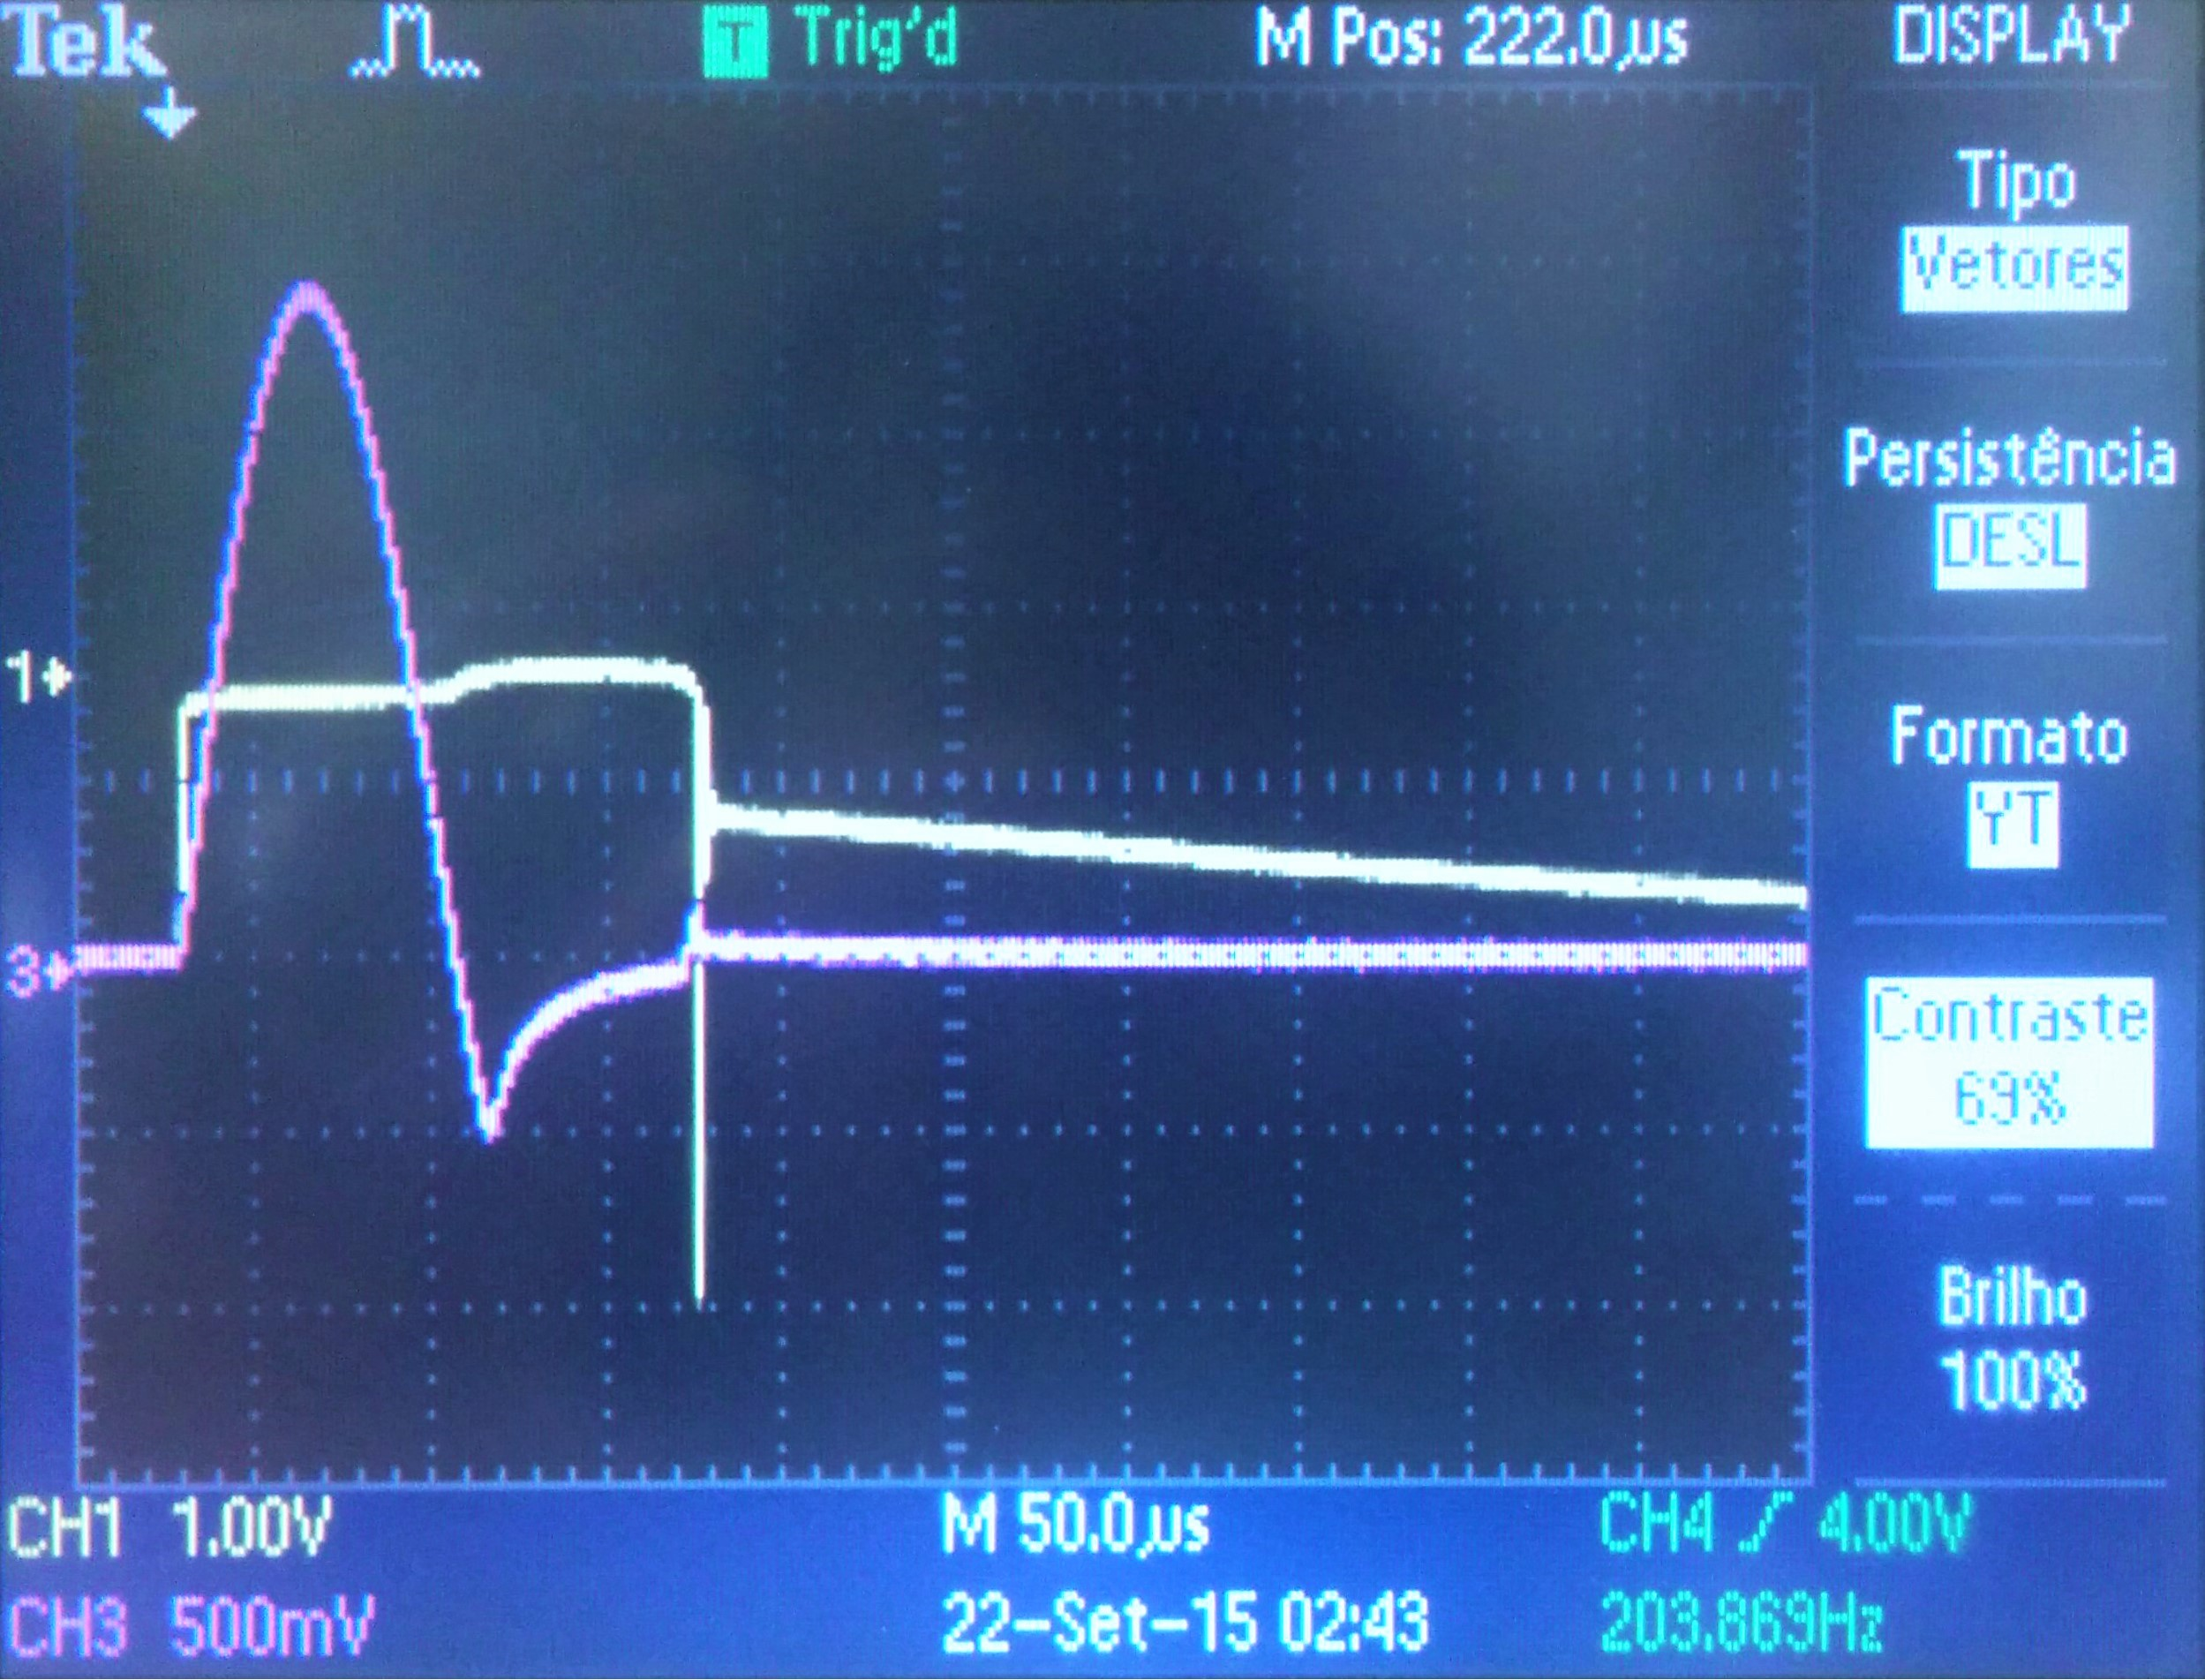
\includegraphics[keepaspectratio=true, scale=0.12]{img/imagem3}
	\caption{Tensão (a amarelo) e corrente (a rosa) no tiristor.}
	\label{fig:imagem3}
	\vspace{-0.8em}
\end{figure}

\pagebreak

Tal como aos terminais do díodo em antiparalelo a corrente durante o período de condução do tiristor apresenta um comportamento sinusoidal, sendo neste caso o da alternância positiva da corrente na bobina, no entanto devido ao atraso da passagem ao corte do tiristor, ainda se pode observar um pouco da alternância negativa.

A tensão aos terminais do tiristor é tal como no caso da secção anterior pois ambos os dispositivos estão em paralelo.

Considera-se no entanto de interesse mencionar o pico de tensão observável em ambos os casos para momento em que o tiristor transita da condução ao corte. Isto deve-se a haver um atraso apreciável na passagem à condução do díodo e ao corte do tiristor, provocando por um instante uma derivada temporal da corrente infinita levando ao pico de tensão.


\subsubsection{Formas de onda da tensão e corrente no díodo lento em antiparalelo}

Ao utilizar o díodo lento em antiparalelo as formas de onda da corrente e tensão são as apresentadas na \autoref{fig:imagem4}.

\begin{figure}[H]
	\centering
	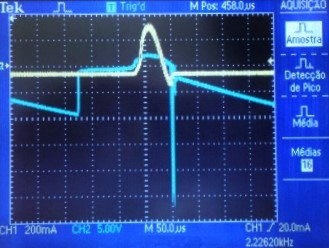
\includegraphics[keepaspectratio=true, scale=1.2]{img/imagem4}
	\caption{Tensão (a azul) e corrente (a amarelo) no diodo lento.}
	\label{fig:imagem4}
	\vspace{-0.8em}
\end{figure}

\subsubsection{Comparação entre o díodo rápido e lento}

Podem fazer-se algumas considerações ao comparar a \autoref{fig:imagem2} com a \autoref{fig:imagem4}.

Em primeiro lugar, nota-se que a tensão V\textsubscript{AK} tem um valor inferior no caso do diodo rápido. Isto deve-se a diferenças no valor da tensão de polarização direta dos dois díodos.

Também se observa que o díodo rápido tem um tempo de condução inferior, pelo que a carga perdida pelo condensador neste caso será também menor.

Por fim tem-se no caso do díodo lento um atraso no tempo de passagem à condução maior, pelo que o período em que se pode observar a arcada negativa da corrente será também maior.

\subsubsection{Funcionamento do circuito}
O funcionamento deste circuito divide-se em três zonas:

\begin{figure}[h]
	\centering
	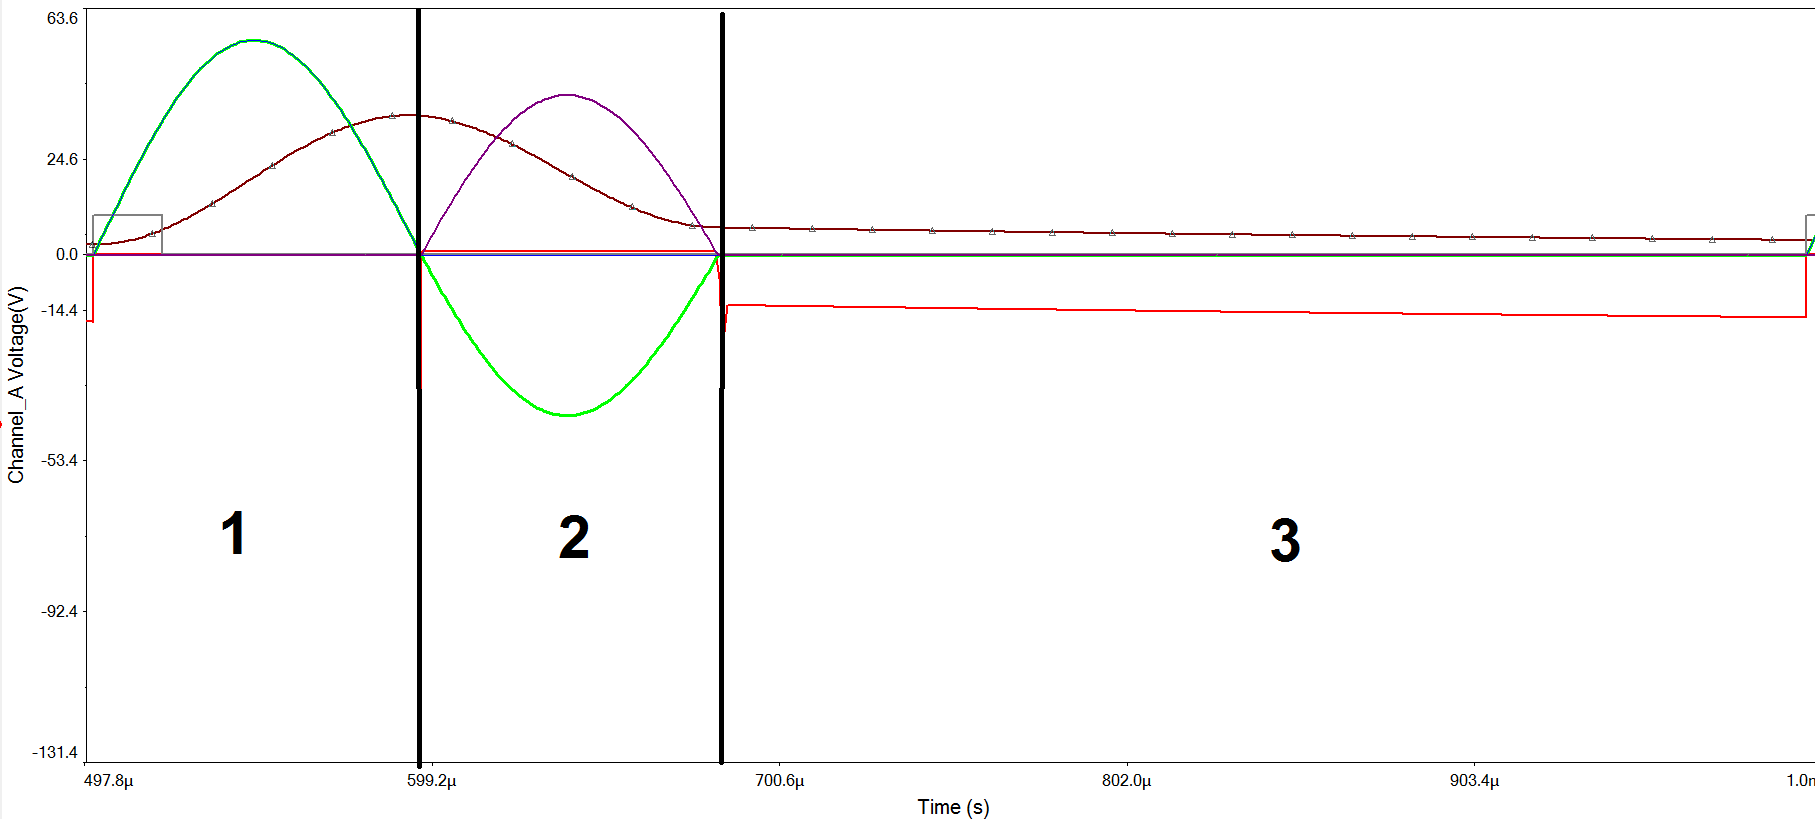
\includegraphics[keepaspectratio=true, scale=0.4]{img/funcionamento_tir}
	\caption{Resultado das simulações.}
	\label{fig:figura 0}
	\vspace{-0.8em}
\end{figure}

\subsubsection*{Zona 1}
	Zona onde o tiristor está a conduzir e o díodo ao corte.
	
	\begin{figure}[h]
		\centering
		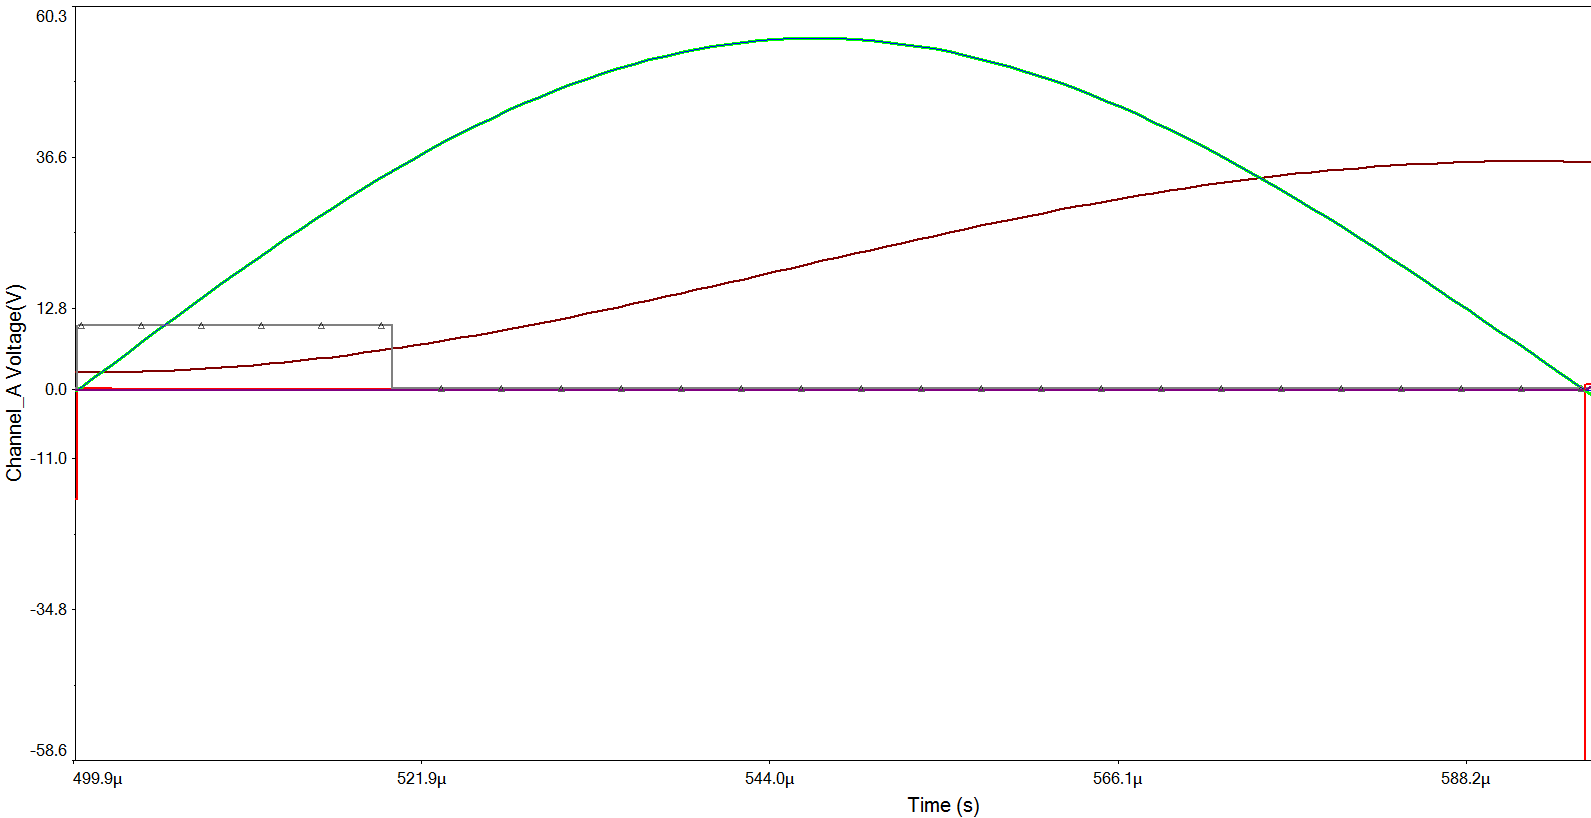
\includegraphics[keepaspectratio=true, scale=0.4]{img/Zona1}
		\caption{Sinal de impluso (cinza), corrente no tiristor (azul), corrente na bobine (verde) e a tensão no condensador (castanho).}
		\label{fig:figura 1}
		\vspace{-0.8em}
	\end{figure}
	
	
	Analisando a simulação verifica-se que quando ocorre o impulso na \textit{gate}, sinal a cinza, a corrente no tiristor tem um comportamento imposto pela bobine, cresce até atingir o seu valor máximo e em seguida decresce até se anular, sinal a verde e sinal a azul. Este comportamento também influência a carga no condensador, como a corrente é no sentido da carga, este carrega até que a corrente se anula, sinal a castanho. Neste ponto o díodo entra em condução.
	
	\pagebreak
	   
\subsubsection*{Zona 2}
	Zona onde o díodo está a conduzir e o tiristor ao corte. 
	
	\begin{figure}[h]
		\centering
		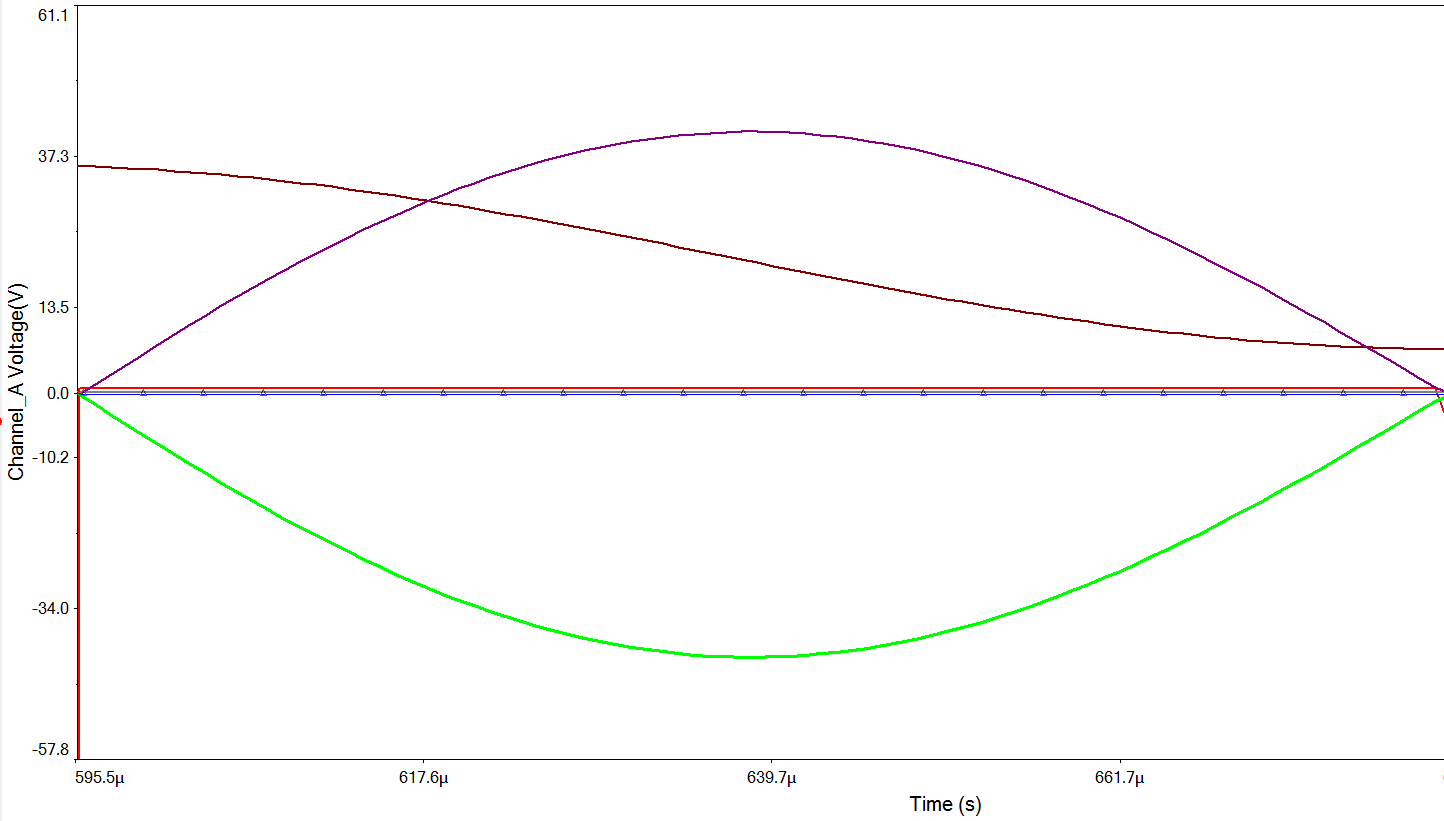
\includegraphics[keepaspectratio=true, scale=0.4]{img/Zona2}
		\caption{Corrente no díodo (roxo), corrente na bobine (verde), tensão no condensador (castanho) e a tensão no tiristor (vermelho).}
		\label{fig:figura 2}
		\vspace{-0.8em}
	\end{figure}
	
	Como já  foi referenciado o tiristor tem um comportamento muito lento no corte. Como o objetivo é abrir o circuito exatamente no ponto em que a corrente no tiristor passa por zero, o tiristor não consegue ter esse comportamento, foi colocado um díodo anti-paralelo de forma a aproximar o corte do zero.    
	
	Com o díodo anti-paralelo a corrente têm o sentido contrário à situação anterior. Com corrente a ter este comportamento é de esperar a descarga do condensador até que a corrente se anula, sinal a castanho Neste ponto o díodo entre em corte.

	
\subsubsection*{Zona 3}
	Zona onde o díodo e o tiristor estão ao corte.
	
	\begin{figure}[h]
		\centering
		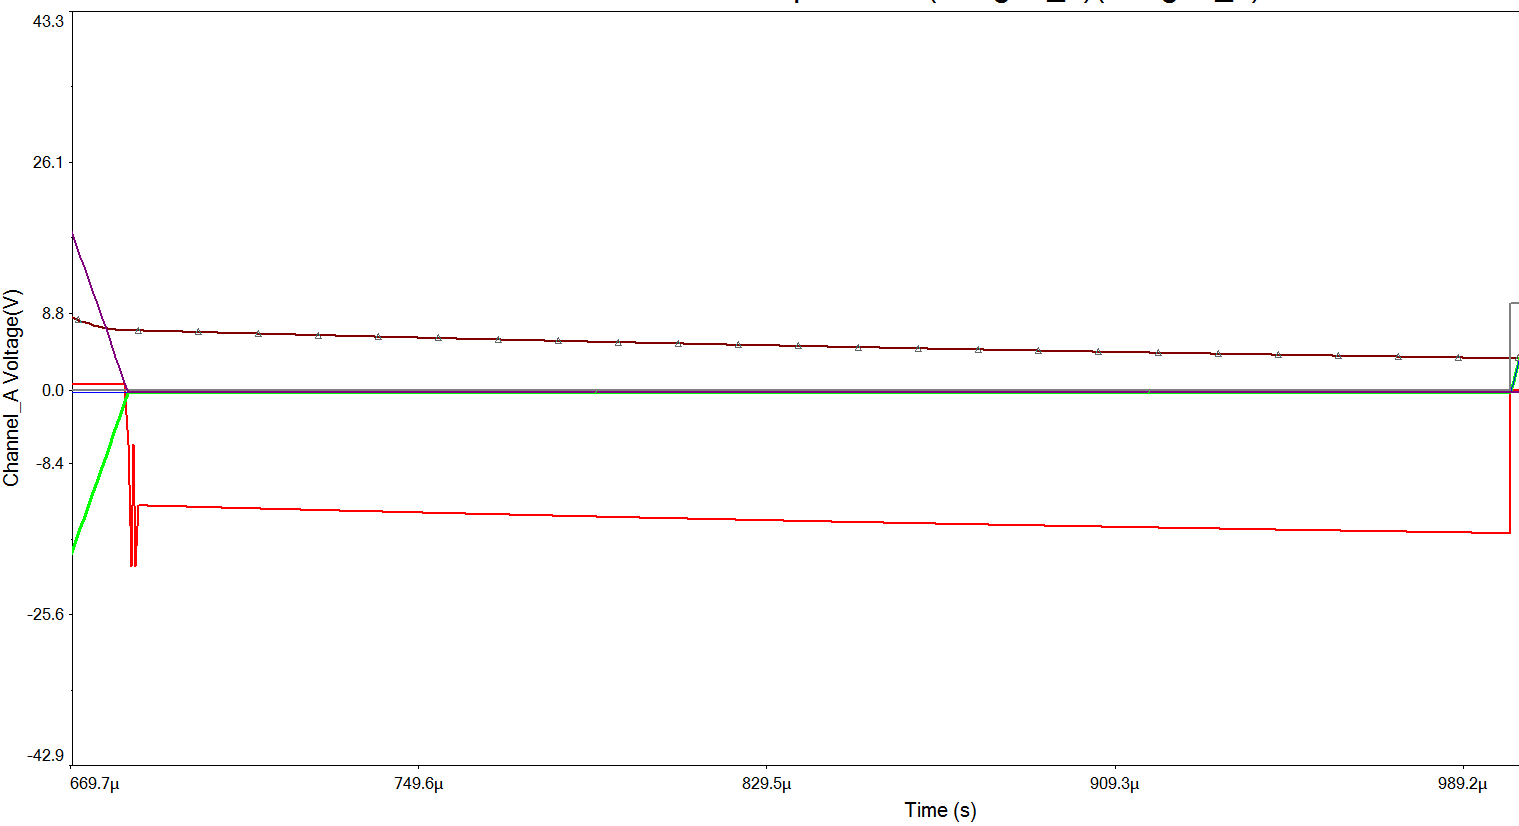
\includegraphics[keepaspectratio=true, scale=0.4]{img/Zona3}
		\caption{Tensão no tiristor (vermelho) e a tensão do condensador (castanho).}
		\label{fig:figura 3}
		\vspace{-0.8em}
	\end{figure}
	
	A corrente na bobine é nula até que haja outro impulso de \textit{gate} de forma a ativar o tiristor. A tensão no condensador decresce até atingir o seu valor mínimo (período de descarga do condensador por entrega de energia à carga).
	
	Os valores máximos de corrente e tensão são determinados pelos parâmetros do circuito de disparo (período do impulso de \textit{gate}) e do circuito de potência (valores da resistência, condensador e bobine).
	A potência entregue à carga é controla através da frequência  do impulso de \textit{gate} (frequência de disparo do tiristor).


\subsubsection{Circuito de potência sem díodo em antiparalelo}
Na \autoref{fig:imagem5} pode ver-se a tensão e corrente no tiristor.

\begin{figure}[h]
	\centering
	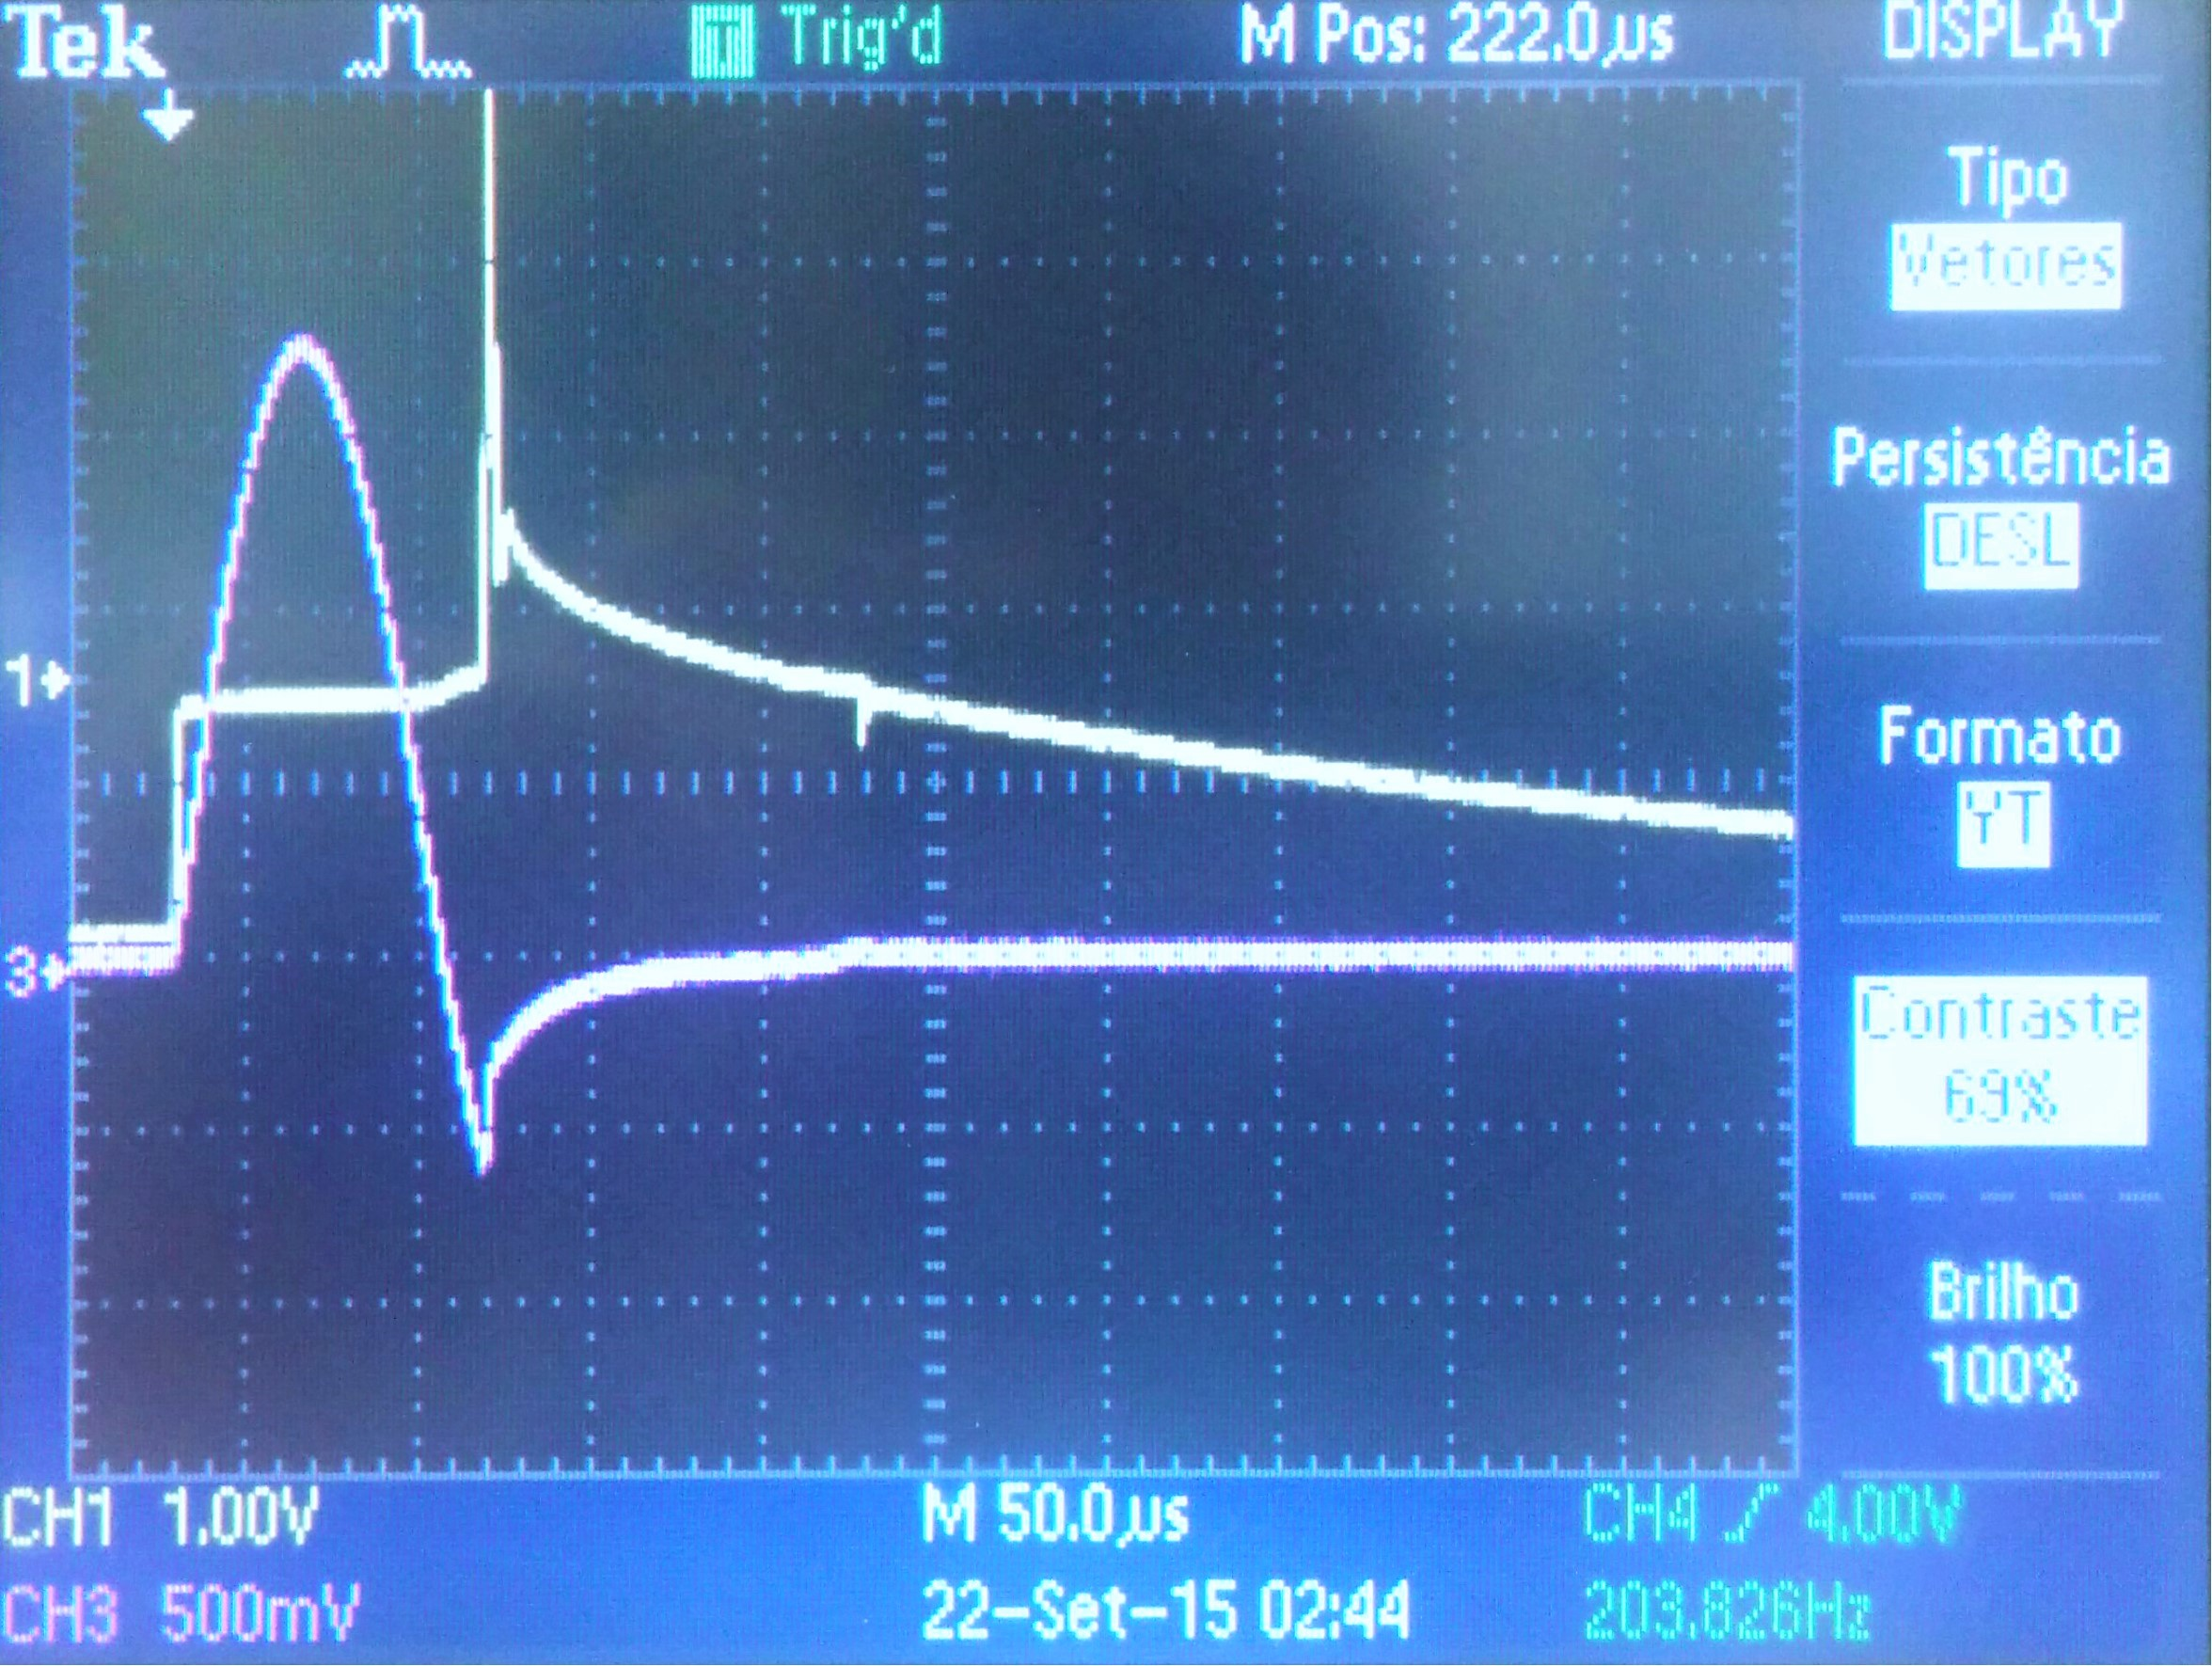
\includegraphics[keepaspectratio=true, scale=0.165]{img/imagem5}
	\caption{Tensão (a amarelo) e corrente (a rosa) no tiristor.}
	\label{fig:imagem5}
	\vspace{-0.8em}
\end{figure}
O sinal a amarelo representa a tensão entre o catado e o anodo, V\textsubscript{KA} e o sinal a rosa representa a corrente no tiristor.
Analisando a figura pode-se dividir o comportamento da tensão em três fases. A primeira fase é definida pela condução do tiristor, a tensão V\textsubscript{KA} é constante e igual à tensão de polarização direta do tiristor, como se pode visualizar no sinal a amarelo. 
A segunda fase representa o momento de corte do tiristor, intervalo desde que a corrente se anula até que o tiristor realmente entra em corte. Pode-se verificar o que já tinha sido referenciado, o tiristor têm um tempo de corte muito elevado. 

Devido à existência da bobine no circuito e corrente neste no momento de corte a tensão  V\textsubscript{KA} tende para infinito, como se pode identificar no sinal amarelo da \autoref{fig:imagem5}. Confirma-se segundo a seguinte expressão:
 
 \begin{equation}
 	\label{eq:ex_1}
 	V = L\,\frac{d}{d\,t}\,i_L + \frac{1}{C}\,\int i_C\,dt
 \end{equation}

Com $i_L = I$ e $i_C = I$ e um $dt = 0$ temos:

 \begin{equation}
 	\label{eq:ex_2}
 	V = L\,\frac{d}{d\,t = 0}\,I + \frac{1}{C}\,\int I\,dt = 0 \Leftrightarrow V \rightarrow \infty
 \end{equation}	

\subsubsection{Circuito de potência sem a resistência de carga}
A inexistência da resistência de carga origina um circuito oscilatório amortecido entre tensão máxima e mínima, 20V e 0V. Este amortecimento deve-se ao facto de o tiristor e o díodo não serem ideias, têm resistências internas.

Se os componentes fossem ideais, a tensão no condensador e a corrente na bobine apresentaria comportamento oscilatório não amortecido.

\subsubsection{Expressão analítica da corrente e da tensão no condensador}

% For future reference, aqui há circuitos fixes de potências: http://www.texample.net/tikz/examples/power-electronics-converter-inverter/

%	\begin{figure}[h]
%		\centering
%		\begin{tikzpicture}
%			\draw
%			(0,0) to[Ty, scale=0.5, transform shape, mirror] (2,0) {}
%			(0,0) -- (0,0.5)
%			(1,0) -- (1,0.5)
%			(2,1) to[D*, scale=0.5, transform shape] (0,1)
%			(0,0) -- (-1,0)
%			(-1,0) to[battery1] (-1,-2)
%			(1,0) -- (2,0)
%			(2,0) to[L] (4,0)
%			(4,0) to[C] (4,-2)
%			(4,0) -- (6,0)
%			(6,0) to[R] (6,-2)
%			(6,-2) -- (-1,-2)
%			(2,-2) node[ground] {}
%			;
%		\end{tikzpicture}
%
%		\caption{Circuito em análise}
%		\label{fig:circuit_e18}
%	\end{figure}

Durante o troço em que o tiristor e o díodo conduzem, a aplicação da lei de Kirchoff das Tensões leva às Equações \ref{eq:KVL_1} e \ref{eq:KVL_2}, e a aplicação da lei de Kirchoff das Correntes leva à Equação \ref{eq:KCL_1}.

\begin{equation}
\label{eq:KVL_1}
V = L\,\frac{d}{d\,t}\,i_L + \frac{1}{C}\,\int i_C\,dt
\end{equation}

\begin{equation}
\label{eq:KVL_2}
R\,i_R = \frac{1}{C}\,\int i_C\,dt
\end{equation}

\begin{equation}
\label{eq:KCL_1}
i_L = i_C + i_R
\end{equation}

Derivando as duas equações da lei das malhas em ordem ao tempo, obtêm-se as Equações \ref{eq:KVL_1d} e \ref{eq:KVL_2d}.

\begin{equation}
\label{eq:KVL_1d}
0 = L\,\frac{d^2}{d\,t^2}\,i_L + \frac{1}{C}\,i_C
\end{equation}

\begin{equation}
\label{eq:KVL_2d}
R\,\frac{d}{d\,t}\,i_R = \frac{1}{C}\,i_C
\end{equation}

Resolvendo o sistema diferencial de segunda ordem, obtém-se um resultado na forma da \autoref{eq:current_simp}.

\begin{equation}
\label{eq:current_simp}
i_L = A\, e^{-\frac{t}{\tau}}\,(B\,\sin{(\omega\,t)}+C\cos{(\omega\,t)}) + I_{L0}
\end{equation}

\begin{equation}
\label{eq:time_constant}
\tau = 2\,R\,C
\end{equation}

\begin{equation}
\label{eq:freq}
\omega = \frac{\sqrt{L\,(4\,R^2\,C-L)}}{2\,R\,L\,C}
\end{equation}


% Isto é a mãe de todas as equações, cabe numa página A2 (sim, A2, não é A3), portanto vai ser estripada, mas fica aqui para referência futura.
%\begin{equation}
%\label{eq:current}
%{{i_L}}\left(t\right)={{e^ {- {{t}\over{2\,C\,R}} }\,\left({{ \left(2\,C\,L\,\left(\left(\left.{{d}\over{d\,t}}\,{{i_L}}\left(t \right)\right|_{t=0}\right)\,C\,L\,R^2+\left({{i_L}}\left(0\right)- {{i_R}}\left(0\right)\right)\,L\,R-\left(\left.{{d}\over{d\,t}}\, {{i_L}}\left(t\right)\right|_{t=0}\right)\,L^2\right)-L\,\left( \left({{i_L}}\left(0\right)-{{i_R}}\left(0\right)\right)\,C\,L\,R- \left(\left.{{d}\over{d\,t}}\,{{i_L}}\left(t\right)\right|_{t=0} \right)\,C\,L^2\right)\right)\,\sin \left({{t\,\sqrt{L\,\left(4\,C\, R^2-L\right)}}\over{2\,C\,L\,R}}\right)}\over{\sqrt{L\,\left(4\,C\,R ^2-L\right)}}}+\left(\left({{i_L}}\left(0\right)-{{i_R}}\left(0 \right)\right)\,C\,L\,R-\left(\left.{{d}\over{d\,t}}\,{{i_L}}\left( t\right)\right|_{t=0}\right)\,C\,L^2\right)\,\cos \left({{t\,\sqrt{L \,\left(4\,C\,R^2-L\right)}}\over{2\,C\,L\,R}}\right)\right)}\over{C \,L\,R}}+{{{{i_R}}\left(0\right)\,R+\left(\left.{{d}\over{d\,t}}\, {{i_L}}\left(t\right)\right|_{t=0}\right)\,L}\over{R}}
%\end{equation}

Quando o tiristor deixa de conduzir (depois da corrente se anular), as equações diferenciais que descrevem o circuito são as mesmas, sendo que a diferença está nas condições iniciais que impõem os valores das constantes.

Quando o díodo deixa de conduzir, $i_L = 0$, pelo que $i_C = -i_R$ e o condensador descarregará exponencialmente graças à resistência. Antes da tensão no díodo caír demasiado, o tiristor volta a disparar, e todo o processo recomeça.

Caso a resistência não existisse, teríamos apenas uma equação diferencial (\autoref{eq:no_resistor}), cuja solução seria a \autoref{eq:current_no_resistor}.

\begin{equation}
\label{eq:no_resistor}
0 = L\,\frac{d^2}{d\,t^2}\,i_L + \frac{1}{C}\,i_L
\end{equation}

\begin{equation}
\label{eq:current_no_resistor}
i_L = I_{L0}\,\cos{(\omega'\,t)} + V_{L0}\,\sqrt{\frac{C}{L}}\,\sin{(\omega'\,t)}
\end{equation}

\begin{equation}
\omega'=\sqrt{C\,L}^-1
\end{equation}

Isto verificar-se-ia quer com o tiristor a conduzir, quer com o tiristor ao corte, e quando o díodo estivesse ao corte, o condensador manteria a sua tensão constante.

\pagebreak

\section{Simulação do Trabalho de Laboratório}
Na figura seguinte está representado o circuito usado para realização da simulação:


\begin{figure}[h]
	\centering
	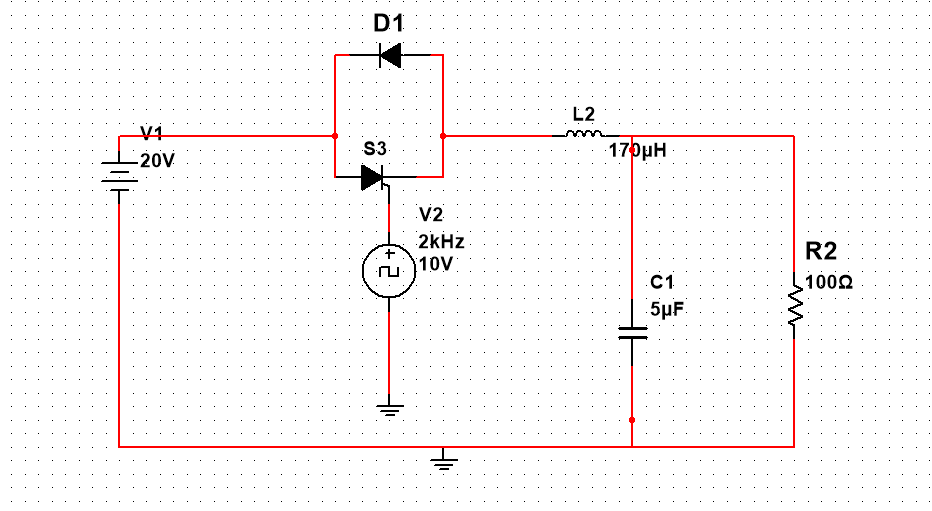
\includegraphics[keepaspectratio=true, scale=0.565]{img/sim/circuit}
	\caption{Circuito para simulação.}
	\label{fig:circ}
	\vspace{-0.8em}
\end{figure}

\subsection{Circuito de disparo}

O circuito de disparo foi simulado usando um gerador de impulsos com 2 kHz de frequência, um factor de ciclo de 2\% e um amplitude de 10 V.

A \autoref{fig:sinal} está representado a seguir:

\begin{figure}[h]
	\centering
	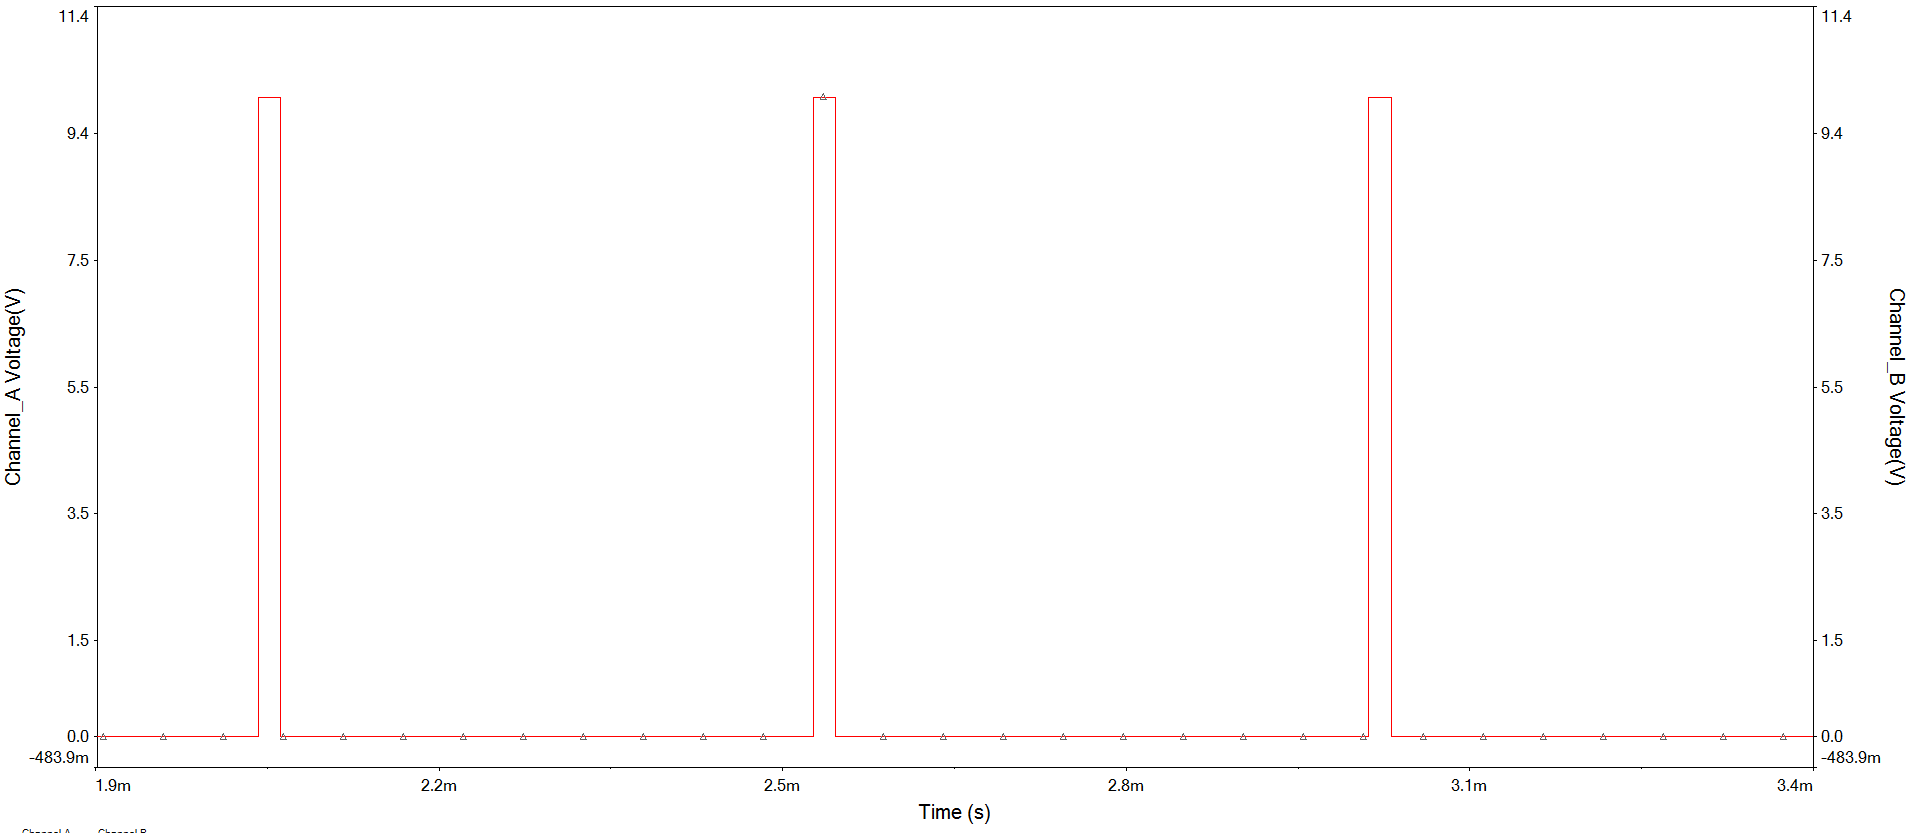
\includegraphics[keepaspectratio=true, scale=0.365]{img/sim/sinalentrada}
	\caption{Sinal de controlo de \textit{gate} em tensão.}
	\label{fig:sinal}
	\vspace{-0.8em}
	\end{figure}
	
\pagebreak

\subsection{Circuito de potência com comutação do tiristor por acção da carga}
\subsubsection{Circuito de potência com díodo em antiparalelo}
 A figura seguinte representa a tensão e corrente no tiristor e no díodo:
 
 \begin{figure}[h]
 	\centering
 	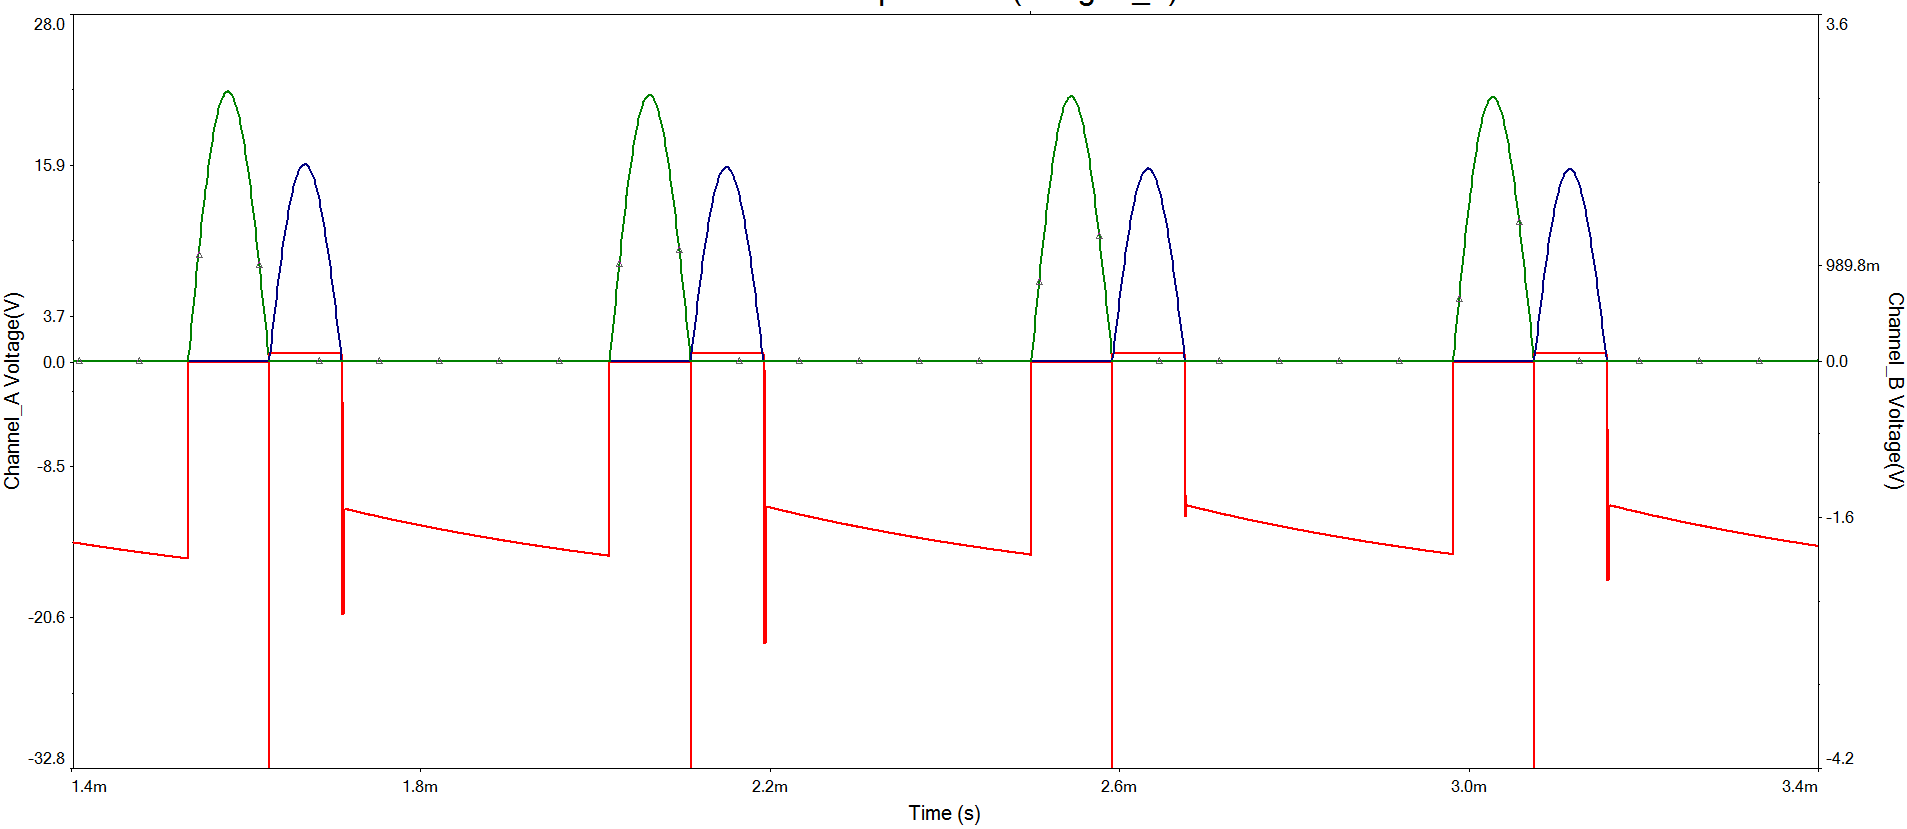
\includegraphics[keepaspectratio=true, scale=0.365]{img/sim/CorrentTensaodiodoeTiristor}
 	\caption{Tensão no tiristor e no díodo (vermelho), corrente no tiristor (verde) e a corrente no díodo (azul).}
 	\label{fig:dio}
 	\vspace{-0.8em}
 \end{figure}
 
 Depois de verificarmos os sinais de corrente e tensão no díodo e no tiristor, pode-se observar os sinais de corrente e tensão na bobine e condensador respetivamente na \autoref{fig:condbobine}.
 
 
 \begin{figure}[h]
 	\centering
 	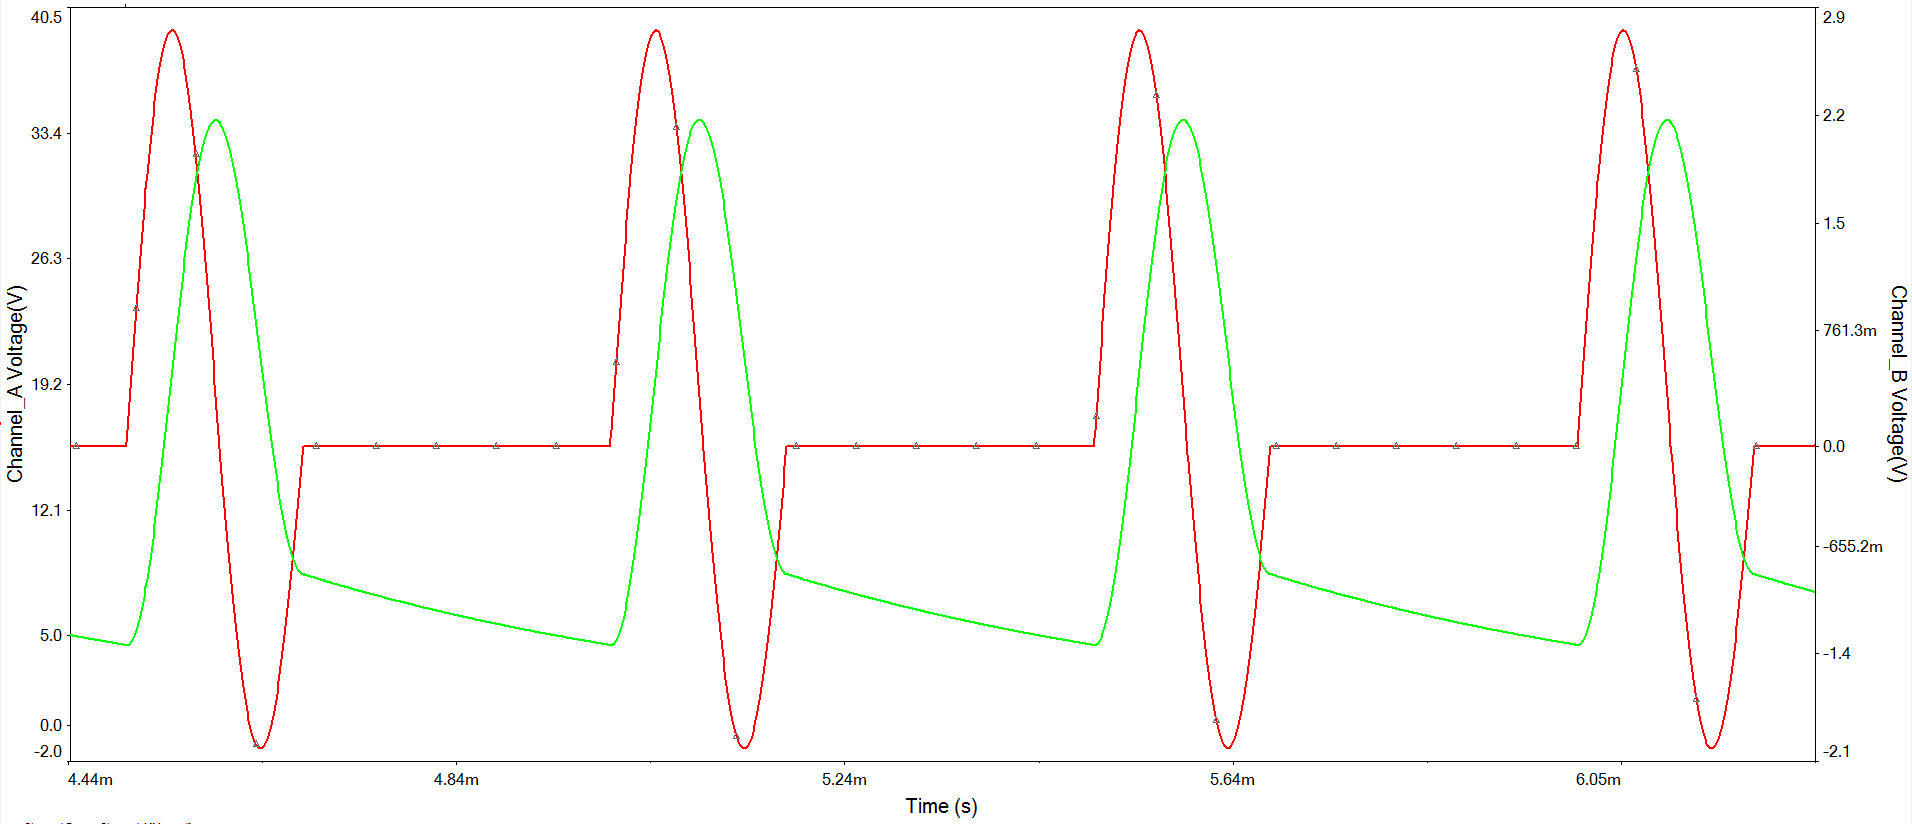
\includegraphics[keepaspectratio=true, scale=0.365]{img/sim/TensaoCondCorrenBobine}
 	\caption{Tensão no condensador (verde) e a corrente na bobine (vermelho).}
 	\label{fig:condbobine}
 	\vspace{-0.8em}
 \end{figure}
 
 \pagebreak
 
\subsubsection{Circuito de potência sem díodo em antiparalelo}
 Na figura seguinte estão representados as formas de onda da corrente e tensão no tiristor.
 
  \begin{figure}[h]
  	\centering
  	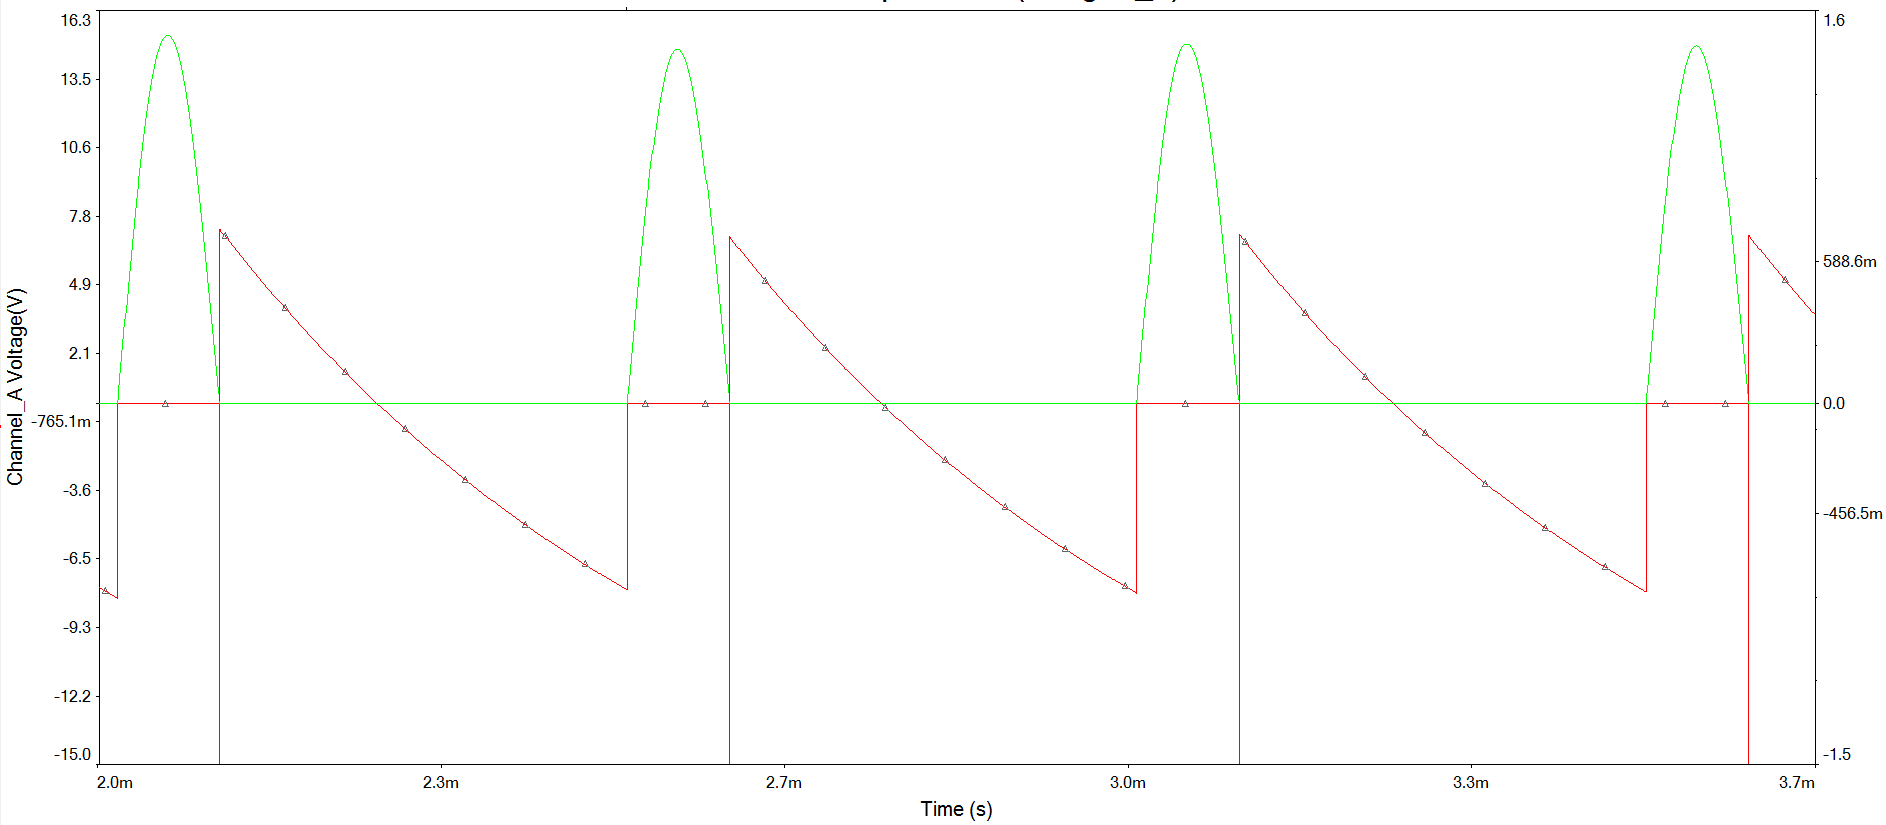
\includegraphics[keepaspectratio=true, scale=0.365]{img/sim/tiristorsemdiodo}
  	\caption{Tensão no tiristor (vermelho) e a sua corrente (verde).}
  	\label{fig:ondbobine}
  	\vspace{-0.8em}
  \end{figure}
  
 Também verificou-se as formas de onda da corrente e tensão na bobine e condensador, respetivamente.
 
  \begin{figure}[h]
  	\centering
  	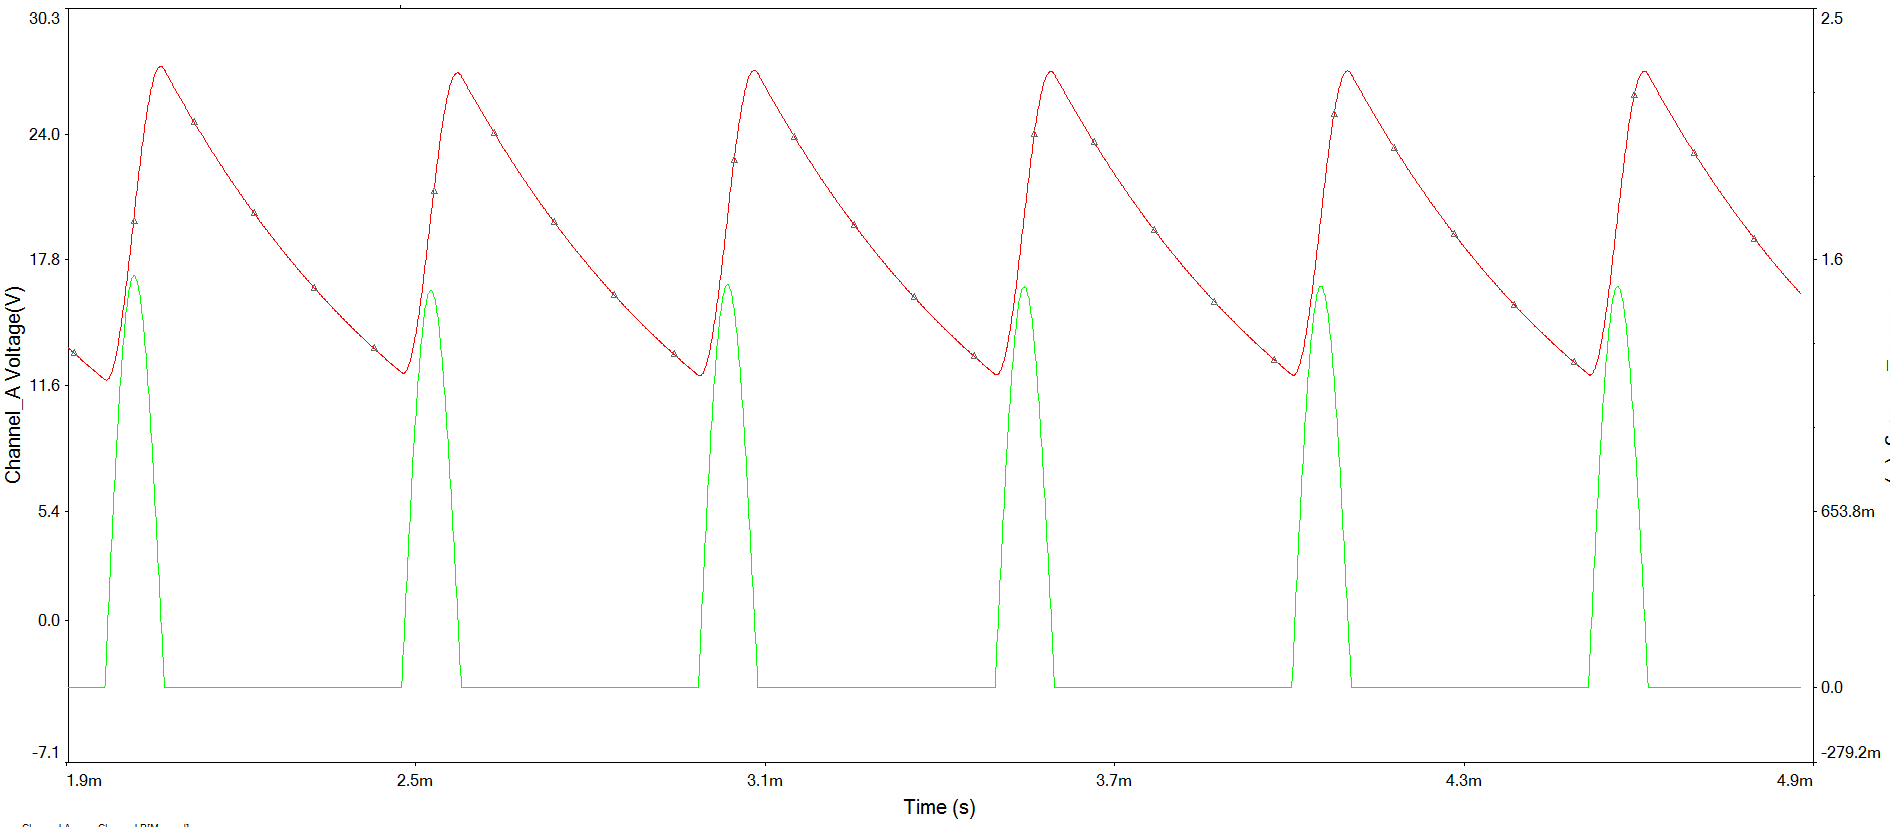
\includegraphics[keepaspectratio=true, scale=0.365]{img/sim/semdiodocond}
  	\caption{Tensão no condensador (vermelho) e corrente na bobine (verde).}
  	\label{fig:bobine}
  	\vspace{-0.8em}
  \end{figure}

\pagebreak

\subsubsection{Circuito de potência sem resitência de carga.}

Pode-se verificar o comportamento oscilatório amortecido visualizado nas formas de onde de corrente e tensão na bobine e condensador respetivamente.

 \begin{figure}[h]
 	\centering
 	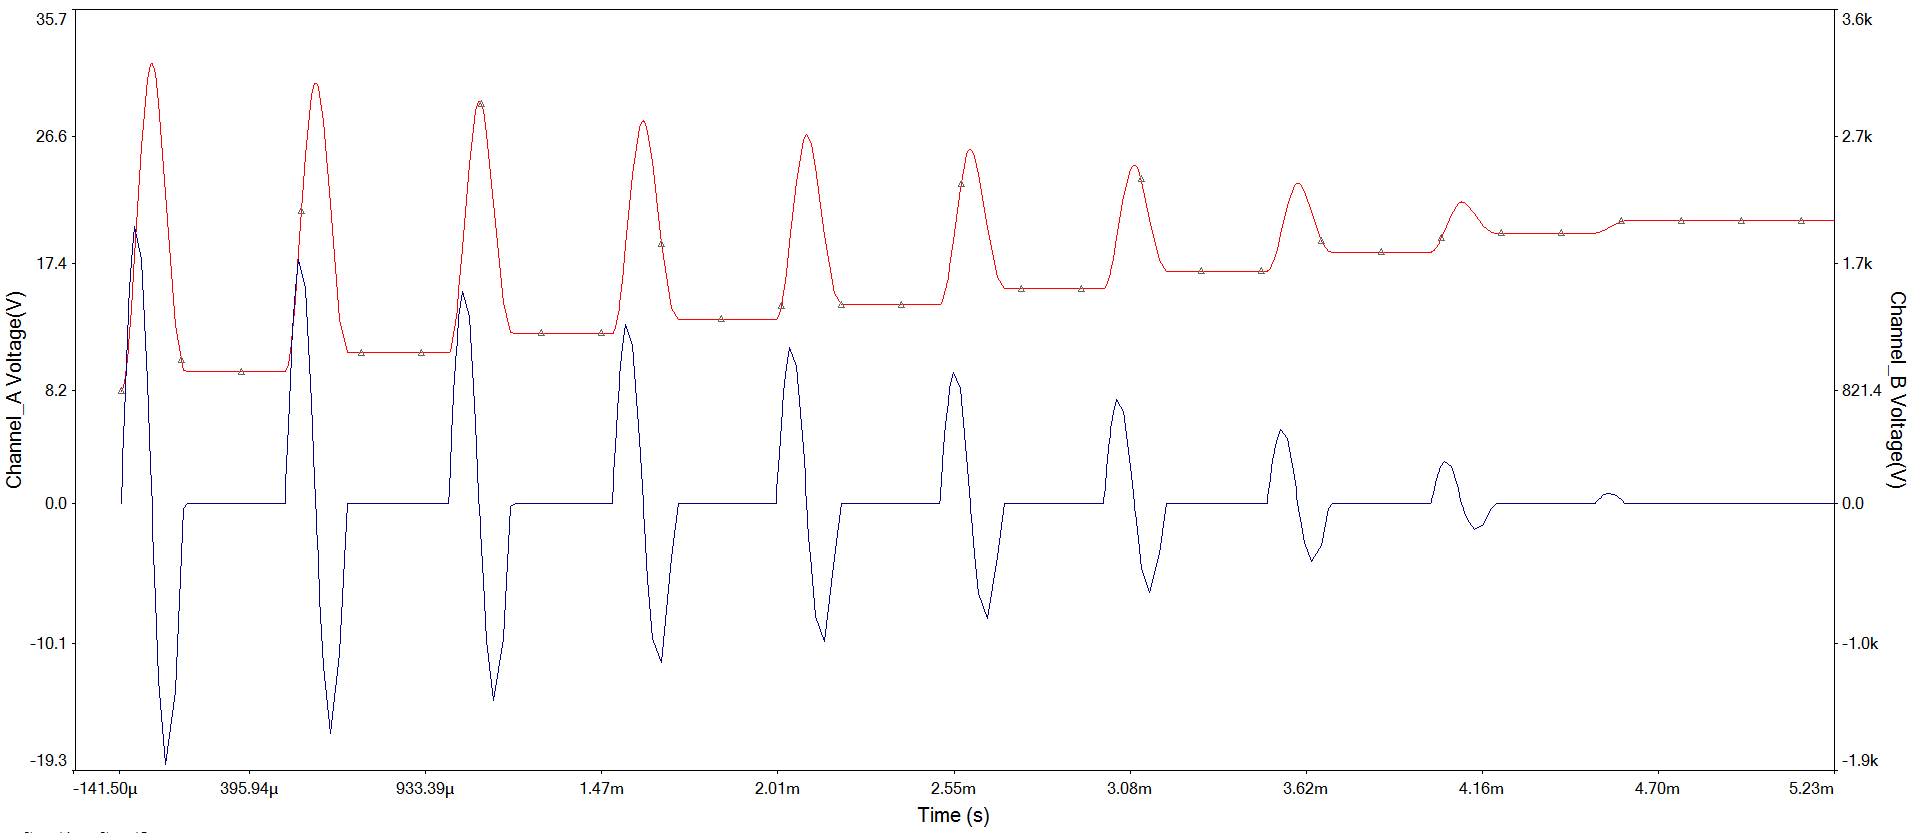
\includegraphics[keepaspectratio=true, scale=0.365]{img/sim/oscil}
 	\caption{Tensão no condensador(vermelho) e corrente na bobine (azul).}
 	\label{fig:conbobine}
 	\vspace{-0.8em}
 \end{figure}

\end{document}
